\documentclass[a4paper,10pt]{article}
%\usepackage[utf8]{inputenc}

\usepackage[T1]{fontenc}

\usepackage[colorinlistoftodos,prependcaption,textsize=tiny]{todonotes}

\usepackage{minted}

\usepackage{blkarray}
\usepackage{amsmath}

\usepackage{hyperref}

%%%%%%%%%%%%%%%%%%%%%%%%%%%%%%%%%%%%%%%%%%%%%%%%%%%%%%%%%%%%%%%%%%%%%%%%%%%%%%%%
% biblatex specific commands
%%%%%%%%%%%%%%%%%%%%%%%%%%%%%%%%%%%%%%%%%%%%%%%%%%%%%%%%%%%%%%%%%%%%%%%%%%%%%%%%

\usepackage[
giveninits=true,
backend=biber,
%style=alphabetic,
sorting=none,
citestyle=numeric,
url=false, 
doi=false,
eprint=false,
isbn=false,
%clearlang=true,
%number=false,
%language=false,
% maxcitenames = 1
]{biblatex}

\renewbibmacro{in:}{%
  \ifentrytype{article}{}{\printtext{\bibstring{in}\intitlepunct}}}

%\DeclareRedundantLanguages{english,german,french}{english,german,ngerman,french}

% \DeclareCiteCommand{\longcite}{}{  %create custom citations awesome indeed !
%     \blx@maxcitenames{1}
%     \printnames[author]{author}, \printfield{year}}{;}{}%

\DefineBibliographyStrings{english}{%
    andothers = {\em et\addabbrvspace al\adddot}
}
% if fields can not be removed due to limitations in the native biber set-up, it can be done by clearing the field itself
\AtEveryBibitem{
\clearfield{month}
\clearlist{language}
\clearfield{number}
\ifentrytype{book}{}{% Remove publisher and editor except for books
  \clearlist{publisher}
  \clearname{editor}
 }
}

% \AtEveryCitekey{
% % \clearfield{month}
% % \clearlist{language}
% % \clearfield{number}
% % \ifentrytype{book}{}{% Remove publisher and editor except for books
% %   \clearlist{publisher}
% %   \clearname{editor}
% % }
% }

 
\addbibresource{./bib/publication.bib} %Imports bibliography file

%%%%%%%%%%%%%%%%%%%%%%%%%%%%%%%%%%%%%%%%%%%%%%%%%%%%%%%%%%%%%%%%%%%%%%%%%%%%%%%%
% biblatex specific commands end
%%%%%%%%%%%%%%%%%%%%%%%%%%%%%%%%%%%%%%%%%%%%%%%%%%%%%%%%%%%%%%%%%%%%%%%%%%%%%%%%


%opening
\title{SSR-viz - a toolbox to detect and visualize protein
subfamily specific residues}
\author{Paul Zierep}

\begin{document}

\maketitle

\begin{abstract}


\end{abstract}

Homologous proteins can be classified into protein families. The members of a family share a similar structure and sequence. Despite their inherent
similarity, individual members of the same family can adopt very specific functions, leading to a further division into subfamilies. These functional
differences can often be assigned to specific residues. This information can be used for various applications, such as function-based subfamily
classification, rational site-directed mutagenesis and general elucidation of mechanisms of action. Here we introduce a novel user-friendly open-source
software which allows for the identification and visualization of these residues.

\pagebreak
\tableofcontents
\pagebreak

\section{What is SSR-viz ?}

SSR-viz helps to detect residues (SSRs) which distinguish protein subfamilies from each other.
Therefore, SSR-viz needs a Multiple Sequence Alignment (MSA) of a protein family and a CSV file which defines the 
subfamilies in the alignment.
For each position in the alignment a score is computed which aims to highlight positions which are conserved in a 
subfamily but differ significantly opposed to another subfamily. 
Various outputs can be created which help to further analyze the detected SSRs.

\section{Installation}

\subsection{Standalone executables}

We implemented standalone 
executables for Windows (tested on windows 10) and Linux (tested on Ubunt 16.04).
These are bigger then the pure python module, but ship everything needed out of
the box. \\

\url{https://github.com/PhaBiFreiburg/SSR-viz/tree/master/standalone/}

\begin{itemize}
\item{Windows: exe.win-amd64-3.5.zip}
\item{Linux: exe.linux-x86\_64-3.5.tar.gz}
\end{itemize}


\subsection{Using Pip}

SSR-viz in implemented as a standalone GUI framework. It is entirely 
written in Python 3. The program was successfully installed on
Ubuntu 14.04/16.04/18.04 and Windows 8/10. It can be installed via PIP - the official python repository. 
To install SSR-viz open a terminal an type: 

\begin{minted}{bash}
pip3 install ssrviz
\end{minted}

Some packages, especially \textbf{wxPython} 
which are normally automatically installed
by PIP can make problems, as they are using system dependencies, which can 
lead to errors when missing. 
Good advice to install wxPython can be 
found at: \url{https://wxpython.org/pages/downloads/index.html}.
They also supply custom builds which work on Ubuntu 16.04 and various other
Linux systems.

Nevertheless, wxPython needs some system dependencies on Linux.
They can be easily installed for Ubuntu 16.04:

\begin{minted}{bash}
sudo apt-get install libwebkitgtk-dev libgtk2.0-dev libsdl1.2-dev \
freeglut3 freeglut3-dev libnotify-dev libgstreamerd-3-dev \
libgl1-mesa-glx libglu1-mesa libgl1-mesa-dev libglu1-mesa-dev \
libgconf2-dev libsdl1.2-dev zlib1g-dev libjpeg62-dev
\end{minted}

In some cases the \textbf{matplotlib} might also need some Help with \textbf{tkinter}.

\begin{minted}{bash}
sudo apt-get install python3-tk
\end{minted}

Installation via Pip for Windows should work without additional installations. \\

Given that installation via pip works for Windows and Linux, chances are good
that SSR-viz might also run on a Mac, but so far we could not make it work,
mainly due to problems with wxPython.

\subsection{Clone from GitHub}

SSR-viz can also be cloned from GitHub \url{https://github.com/PhaBiFreiburg/SSR-viz}.
But then the dependencies need to be installed manually, 
see: \\
SSR-viz/documenation/requirements.txt

\subsection{Mafft}

The only external tool needed is mafft, an excellent alignment tool which is 
required to map protein structure indices to the alignment. SSR-viz runs
without mafft, but for the \textbf{Add\_pdb} tool the mafft executable needs 
to be assigned (see Section~\ref{mafft} for further help).
Dont't worry mafft is easy to install on all systems:

\url{https://mafft.cbrc.jp/alignment/software/}

\section{Getting started}

In Section~\ref{example} a detailed use case is demonstrated, which shows
the usage of each tool as well as the input and output formats.
The use case can be reproduced with the provided files in
 \url{https://github.com/PhaBiFreiburg/SSR-viz/use_case}.

The SSR-viz algorithm is based on a multiple sequence alignment (MSA) file in 
FASTA format, which can be generated with various tools, such as Clustalo 
and Mafft or with a Webserver such as 
\href{https://zeus.cmm.msu.ru/#scenario=2}{Mustguseal} or 
\href{http://prodata.swmed.edu/promals3d/promals3d.php}{PROMALS3D}.

The topic of sequence alignment is beyond the scope of this manual.  
Nevertheless one should keep in mind that 
the quality of the alignment is crucial for the detection algorithm.
(Is is difficult to interpret the importance of a position, which has
more gaps then amino acids.)

Please provide the alignment in FASTA format, most tools allow this format as
an output option.

The first step is the classification of the sequences into subfamilies.
This is undoubtedly the most difficult part, as it often requires 
to identify the specific functionality based on scientific literature
or even undertake experimental validation. Dedicated databases such as 
\href{https://www.uniprot.org/}{UniProt} and \href{http://www.pantherdb.org/downloads/index.jsp}{PANTHER} 
can help to identify 
detailed protein functionality. 

Even though there are various tools available that can cluster protein sequences, 
these clustering methods always apply some kind of similarity scoring,
which leads in most cases to a clustering based on evolutionary relationship 
rather then functional similarity. 
This is demonstrated on an example in Section~\ref{example}.

Ones you collected the class information of your sequences you can add
them to your alignment. The \textbf{CSV\_Builder} tool allows to creates 
a comma separated value (CSV) file which can be used to add the subfamily 
class label to the sequences
(see section~\ref{csv_b}).

An alignment and the CSV file is everything needed to 
detect subfamily specific residues in the sequences. 
The \textbf{SSR\_plot} tool handles the actual execution of the detection
algorithm, the output can be a mathplotlib \cite{hunter_matplotlib:_2007} style plot (see section~\ref{ssr_p})
as pdf, a Javlview annotation file \cite{clamp_jalview_2004} (which can show the results together with the 
alignment) as well as a 'stats.csv' file which summarizes the SSRs.

In most cases it is desired to observe the SSRs in a structural context.
Therefore, we also developed a tool \textbf{Add\_pdb} which allows
to map the indices of a protein structure file (*.pdb) to the indices of the 
alignment in the 'stats.csv' file (see section~\ref{add_p}).

An overview chart which explains the setup of the three tools is shown in
the figure~\ref{fig:flow_chart}.

\begin{figure}
  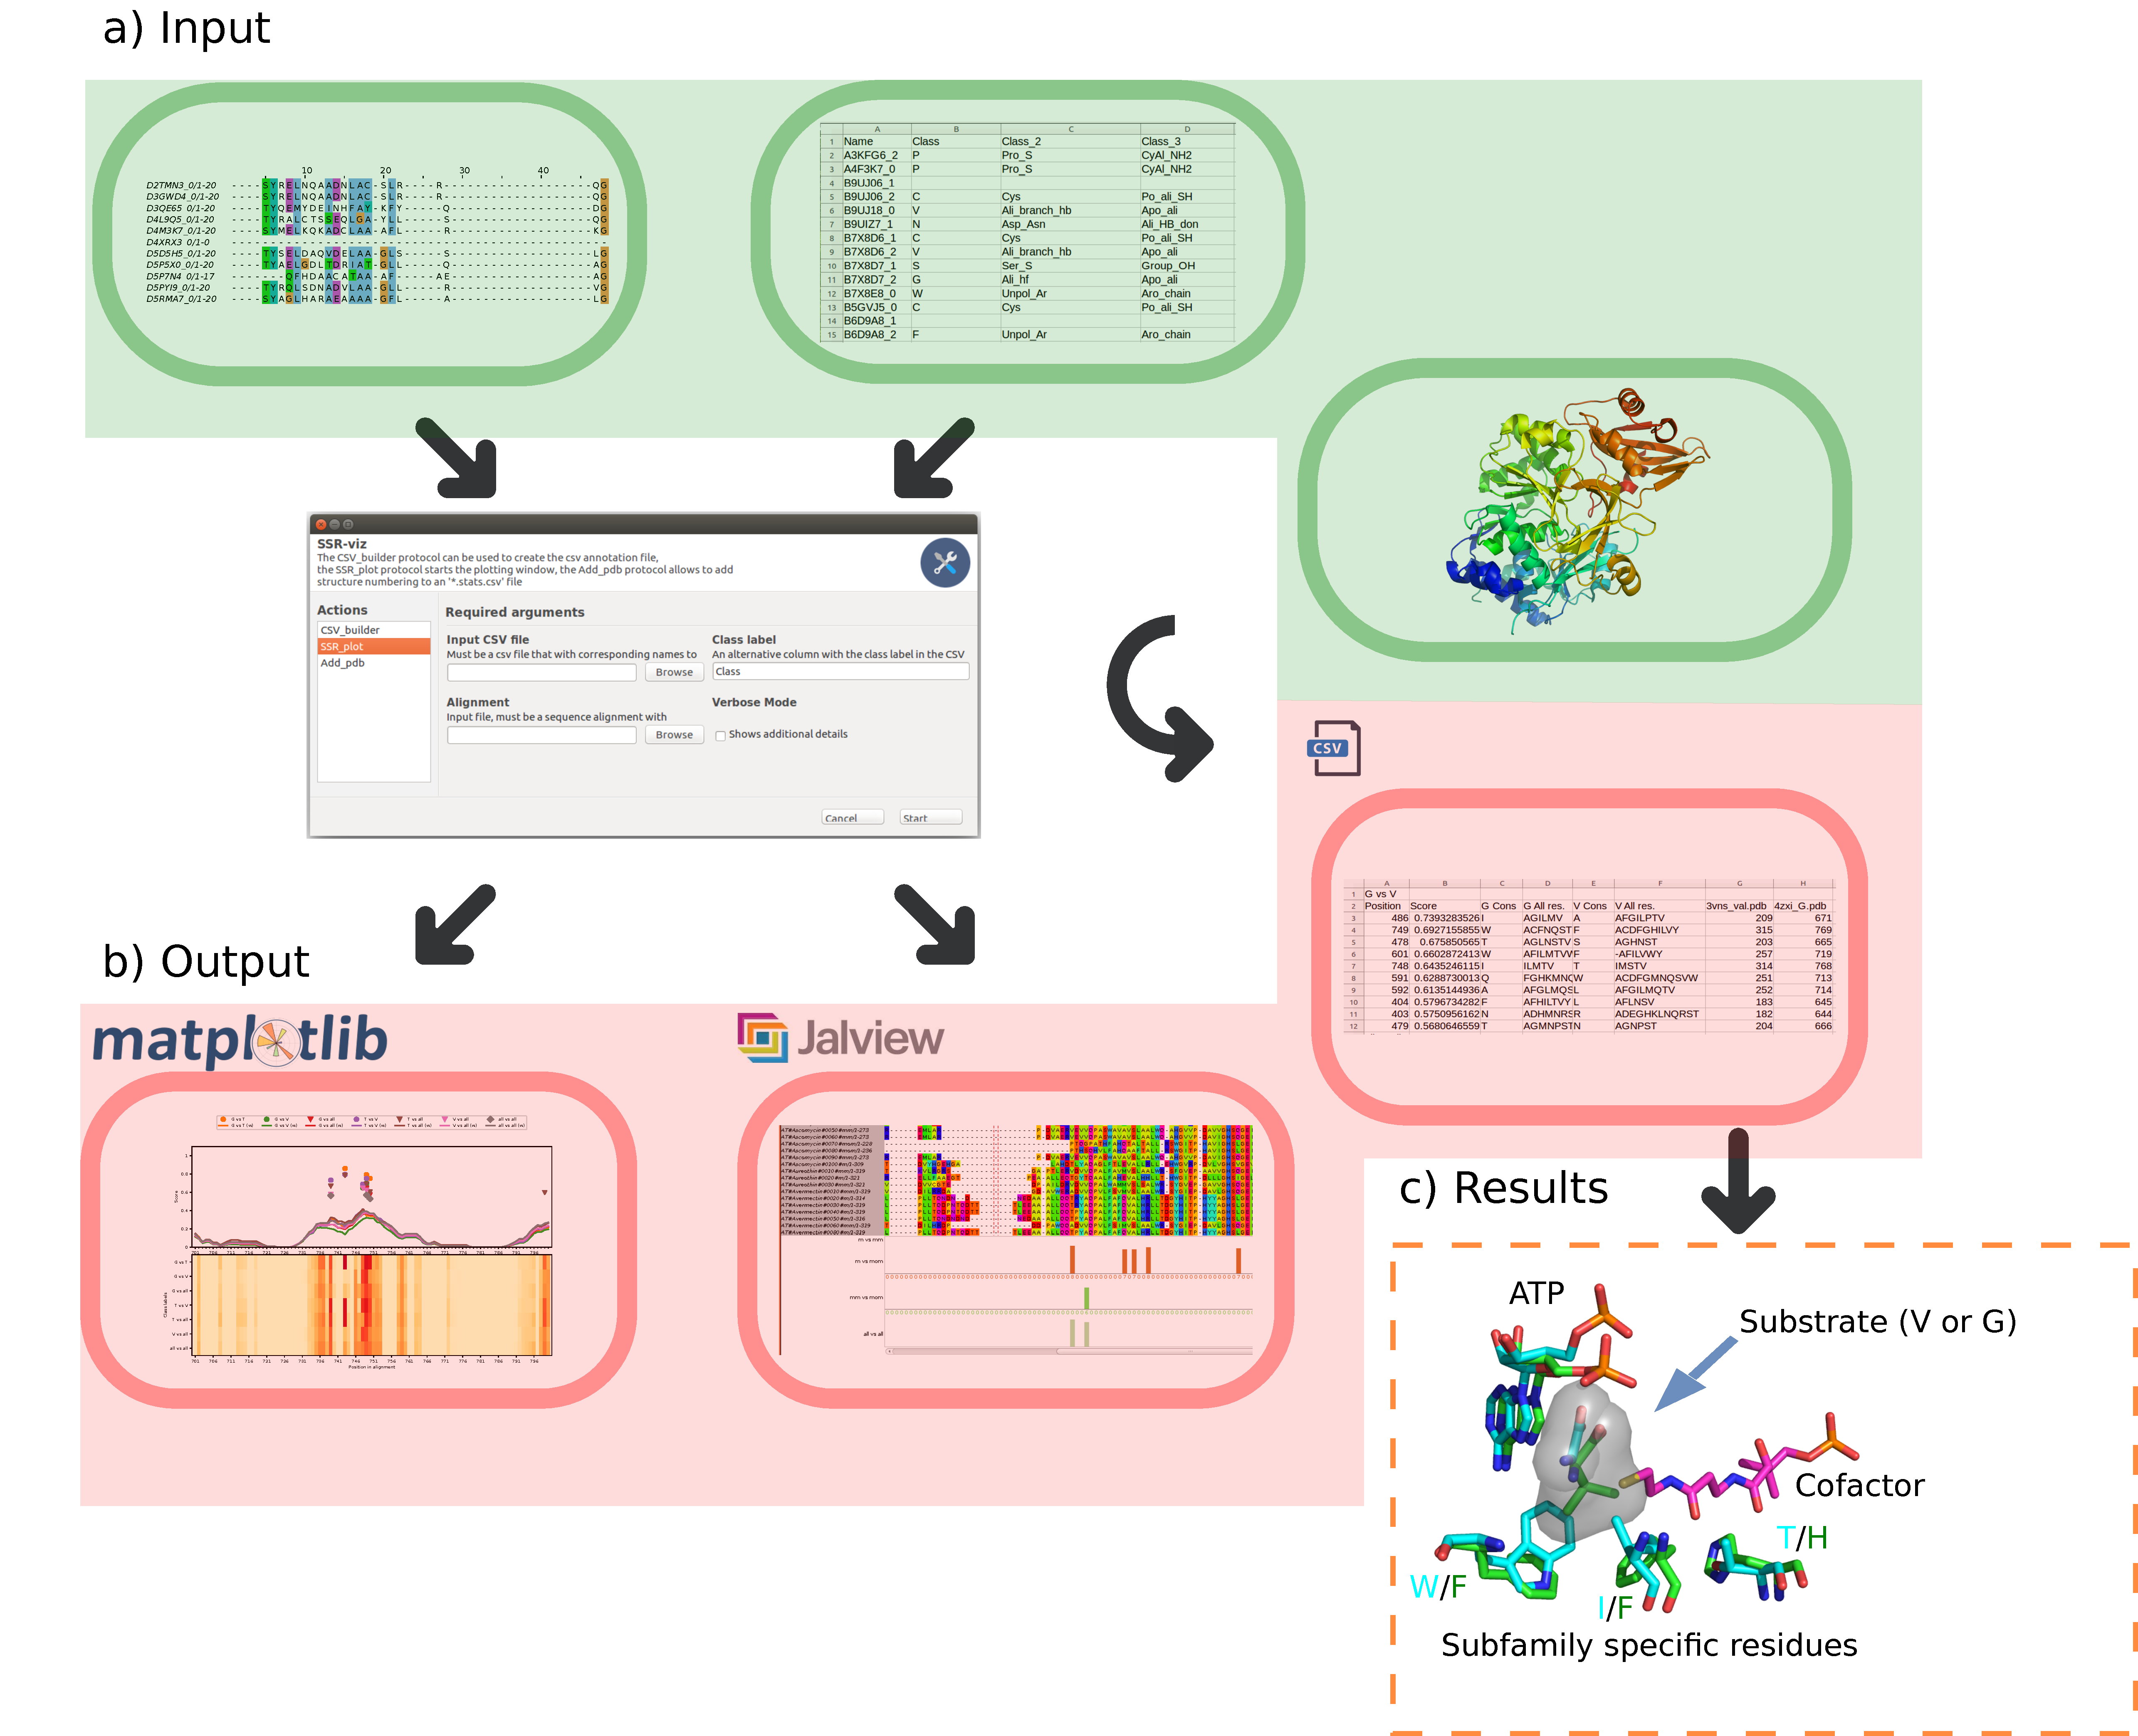
\includegraphics[width=\linewidth]{./figs/flow_chart}
  \caption{General flow chart of the SSR-viz toolbox. a) The input consists 
of a MSA together with a CSV-file holding the corresponding subfamily class labels. 
Multiple protein structures can also be included in order to assign the 
structure indices. b) The output can be created as a mathplotlib PDF, a Jalview annotation file
or a summary CSV-File. This file is used to assign the indices of the structure.
c) Example assignment of SSRs for the NRPS adenylation domain with specificity for Valine and Glycine.}
  \label{fig:flow_chart}
\end{figure}

\section{Algorithm} \label{algo}

The alignment is split into groups representing each protein subfamily as defined in the 
subfamily class label CSV file.
For each group a position probability matrix (PPM) is generated (see eq.\ref{eq:ppm}).
This represents the alignment in form of the probability to find each amino acid at a certain position.
In the following equations $\alpha$ and $\beta$ represent PPMs for two different subfamilies. 

\begin{equation} \label{eq:ppm}
PPM(\alpha) =
\begin{blockarray}{cccc}
 & 1 & 2  & m  \\
\begin{block}{c(ccc)}
  A & \alpha_{A1} & \alpha_{A2}  & \alpha_{Am} \\
  R & \alpha_{R1} & \alpha_{R2}  & \alpha_{Rm} \\
  n & \alpha_{n1} & \alpha_{n2}  & \alpha_{nm} \\
\end{block}
\end{blockarray}
\end{equation}

The conservation score (CS) for each group is computed by applying the normalized Shannon entropy
for each subfamily (eq.\ref{eq:sen}). The score is inverted so that 1 represents a highly conserved position and 0
a not conserved position (eq.\ref{eq:inv}). The mean of both subfamily represents the final CS (eq.\ref{eq:e_comp}).

\begin{equation} \label{eq:sen}
S(\alpha)_m = -\frac{\sum(\alpha_n*\log_2(\alpha_n))}{S_{max}}
\end{equation}

\begin{equation} \label{eq:inv}
CS(\alpha)_m = 1 - S(\alpha) 
\end{equation}

\begin{equation} \label{eq:e_comp}
CS(\alpha, \beta)_m = \frac{CS(\alpha)_m + CS(\beta)_m}{2}
\end{equation}

The difference of both subfamilies is represented by computing an 
exchange probability matrix of both PPMs (eq.\ref{eq:diff}).
This represents the probability of each residue to be exchanged with another
residues in the other subfamily. The sum of the matrix results in the
exchange probability (EP) score.

\begin{equation}  \label{eq:diff}
EP(\alpha,\beta)_m =
  \sum \sum
  \begin{bmatrix}
    0 & \alpha_{A1} * \beta_{R1} & \alpha_{A1} * \beta_{n1} \\
    \alpha_{R1} * \beta_{A1} & 0 & \alpha_{R1} * \beta_{n1} \\
    \alpha_{n1} * \beta_{A1} & \alpha_{n1} * \beta_{R1} & 0 \\
  \end{bmatrix}
\end{equation}

In order to highlight residues which are exchanged with
residues with different physico-chemical properties, an additionally
score is introduced. Therefore, a weighed exchange matrix (WEM)
is computed based on traditional substitution matrices such as PAM and BLOSUM (eq.\ref{eq:we}). 
The matrix can be chosen as a parameter in the algorithm options.

Based on this matrix the weighed exchange probability (WEP) is computed by multiplying the
EP with the matrix, thereby weighing the exchange differently based on the factor of the WEM (eq.\ref{eq:wep}).
This score is additional weighed with a factor $\gamma$ in order to allow users to define the strength of the 
WEM individually. For some experiments a stronger focus on residues with physico-chemical exchange might be desired.

\begin{equation}  \label{eq:we}
WEM =
\begin{blockarray}{cccc}
 & A & R  & n  \\
\begin{block}{c(ccc)}
  A & 0 & i_{AR}  & i_{An} \\
  R & i_{RA} & 0  &  i_{An} \\
  n & i_{nA} &  i_{nR}  & 0 \\
\end{block}
\end{blockarray}
\end{equation}

\begin{equation} \label{eq:wep}
WEP(\alpha,\beta)_m = \sum\sum (EP(\alpha,\beta)_m * WEM) * \gamma
\end{equation}

The final subfamily specific residue (SSR) score of position m ($ES_m$) is computed by 
summation of all three individual scores.
\begin{equation}
SSR_{score}(\alpha, \beta)_m = CS(\alpha, \beta)_m * EP(\alpha, \beta)_m * WEP(\alpha, \beta)_m 
\end{equation}

An example of the scoring algorithm for a hypothetical alignment can be seen in figure~\ref{fig:scoring_02bigger}.

\begin{figure}
  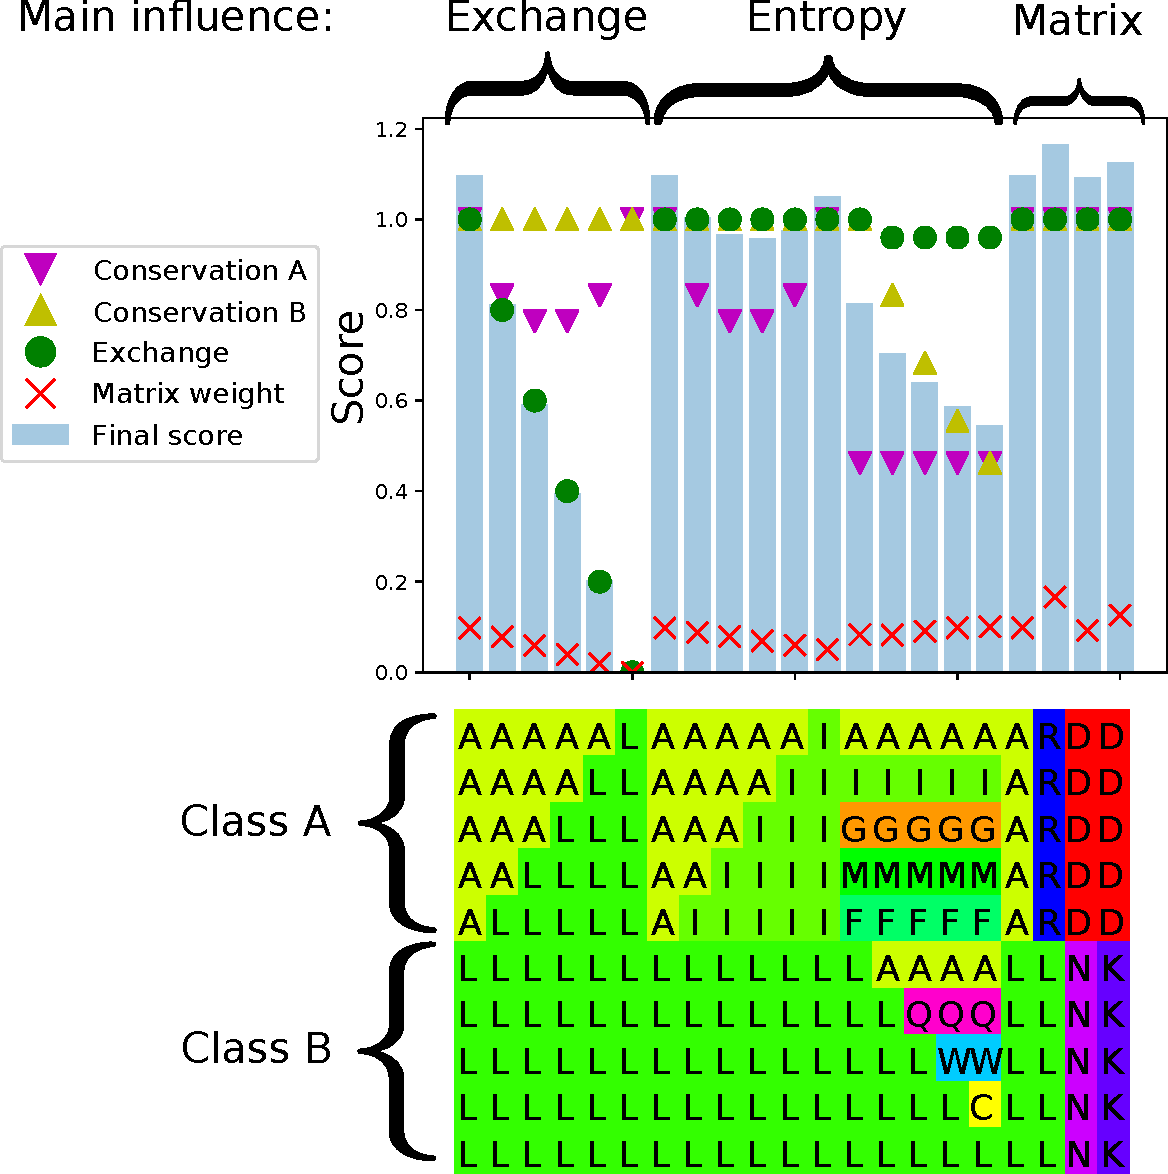
\includegraphics[width=\linewidth]{./figs/scoring_02bigger}
  \caption{Influence of the different scores for a hypothetical alignment of two protein subfamily classes. On top the main 
  influence is indicated: The exchange of an amino acid between the subfamilies (Exchange), the influence of
  the entropy inside a subfamily (Entropy) and the influence of an amino acid exchange of different 
  types of amino acids (Matrix). The default parameters of SSR-viz were used for this example.
  }
  \label{fig:scoring_02bigger}
\end{figure}

\section{CSV builder} \label{csv_b}

The \textbf{CSV\_Builder} handles the input and takes care, 
that the alignment and CSV class label file have the right formating.

\subsection{Arguments}

\begin{description}

\item[\texttt{Input sequence alignment file}] \hfill \\
 
The alignment file with the sequences of the family.
The desired format is in FASTA format (clustalo), see section~\ref{example}
for an example.

\item[\texttt{Inplace FASTA conversion / Temporary alignment file name}] \hfill \\
 
The \textbf{CSV\_Builder} routine will remove duplicates from the 
alignment, as multiple identical sequences will overestimate the importance
of this subfamily. The alignment can be converted inplace, meaning
the original alignment is overwritten or a new alignment can be 
created.

\item[\texttt{Regex extraction of the class label}] \hfill \\
 
The normal \textbf{CSV\_Builder} routine will create a CSV file,
with an empty column for the class labels. Which must be manually 
filled.
In some cases the class labels are part of the sequence names,
this labels can be extracted using regular expressions (regex) patterns.
The entire scope of regex is to big for this manual, but the set of
examples in the appendix~\ref{appendix} should help to get started. There are various 
tools available which can be used to test regex before usage, most text editors 
support regex as a search option. You can 
for example load the alignment file into sublime or notepad, then
search with regex and if the pattern is correct, it should only highlight 
the desired class label. An example is shown in appendix~\ref{appendix}.

\item[\texttt{Output}] \hfill \\

The name of the CSV file, by default it will be created in the same folder as
the sequence file.

\item[\texttt{Delete}] \hfill \\

Allows to overwrite existing CSV files.

\end{description}

\section{SSR plot} \label{ssr_p}

As soon as the alignment file and the class label csv file are created, the detection of
significant SSRs can be performed. 
Therefore, the alignment and the CSV file need to be loaded with the SSR\_plot panel,
if they are loaded correctly, an additional window will open, which allows to set the parameters 
for the detection algorithm and the output options.

\subsection{Arguments}

\begin{description}

\item[\texttt{Input CSV file}] \hfill \\
 
The CSV file holding the class labels. 

\item[\texttt{Class label}] \hfill \\
 
The name of the column holding the subfamily class label information, normally this should just be called "Class",
but an alternative column name can also be chosen, in order to use alternative class definitions. See also:
\ref{example}.

\item[\texttt{Alignment}] \hfill \\

The alignment file used to create the CSV file. Different alignments can be chosen in oder to 
observe influence of the alignment parameters or the alignment algorithm. But the names of the sequences in 
the file need to match the names in the CSV file.

\item[\texttt{Verbose}] \hfill \\

Shows some additional informations about the loading process, for example which files do not match between CSV and alignment file.
(Ideally this should not happen.)

\end{description}

\section{SSR draw} \label{ssr_p}

In this new window all parameters for the algorithm and the output can be adjusted. Each time the start button is pressed
the SSRs are computed based on the current parameters.

Most of the arguments are self-explanatory, therefore only the more advanced options will be explained in the following
argument list.

\subsection{Arguments}

\subsubsection{File}

\begin{description}

\item[\texttt{File name}] \hfill \\

In many cases it is useful to compute multiple plots and files in order to compare the output with each other.
The computed files have the "file name" argument as prefix. Various runs can be performed
successively by tuning the parameters and changing the file name for each run.
 
\end{description}

\subsubsection{Algorithm}

Here the basic parameters for the algorithm can be set, see also \ref{algo}.

\begin{description}

\item[\texttt{Outliers threshold}] \hfill \\

In order to detect the most significant positions a detection threshold can be set, based on the Z-score,
see \url{https://en.wikipedia.org/wiki/Standard_score}. 
 
\item[\texttt{Best positions}] \hfill \\

A more simple, but less significant approach to filter the most important SSRs can be done by simply setting a 
threshold for the best positions, this approach will always return a set of residues. 

The Z-score and Best positions argument can also be set together.

\item[\texttt{Gap importance}] \hfill \\

The implemented algorithm considers gaps as a kind of special amino acid, they are assigned a positions in the replacement matrices.
It is difficult to judge the importance of gaps for the detection of SSRs. For example, if a conserved position in protein class A, is 
exchanged with a gap in protein class B, this could be an important information or it could be due to the alignment algorithm.
Therefore, we decided to let the user judge the gaps individually. If the "gap importance" is set to 0, an exchange with an gap will be considered as
unimportant. If the "gap importance" is set to 1 it is considered as an most important amino acid exchange. The influence of the gap can be judged
by running the algorithm with both settings each and comparing, if the significant positions are changed.

\item[\texttt{Matrix}] \hfill \\

This allows to choose the substitution matrix used for the algorithm (see~\ref{algo}), all matrices which are implemented in Biopython can be used,
see \url{http://biopython.org/DIST/docs/api/Bio.SubsMat.MatrixInfo-module.html} for details. 

Additionally, we computed a substitution matrix purely based on the physico-chemical properties of the amino acids, 
based on \cite{chrysostomou_novel_2015}. 

\item[\texttt{Weight of the replacement matrix}] \hfill \\

The basic algorithm computes the most significant residues to distinguish protein subfamilies. 
Amino acid properties are not considered for this analysis. In many cases
even residues which are very similar can have a great influence on protein function, in other cases
the have no influence at all. Therefore, we allow the user to decide how important the substitution matrix should be
weighed. 
The default parameter of 0.01 is usually a good start. This will only little influence the initial order of the residues,
but for those residues with the same score, they will be reordered with a higher focus on residues replaced with more different residues.
See also \ref{algo} and \ref{example}.

\end{description}

\subsubsection{Figure}

Here the created visualization can be adjusted, in order to create nice looking plots.
The output figure consists of two parts, a heatmap of the SSRs and a plot 
with the most significant positions on top (see figure \ref{fig:plot_example}).
 
\begin{figure}
  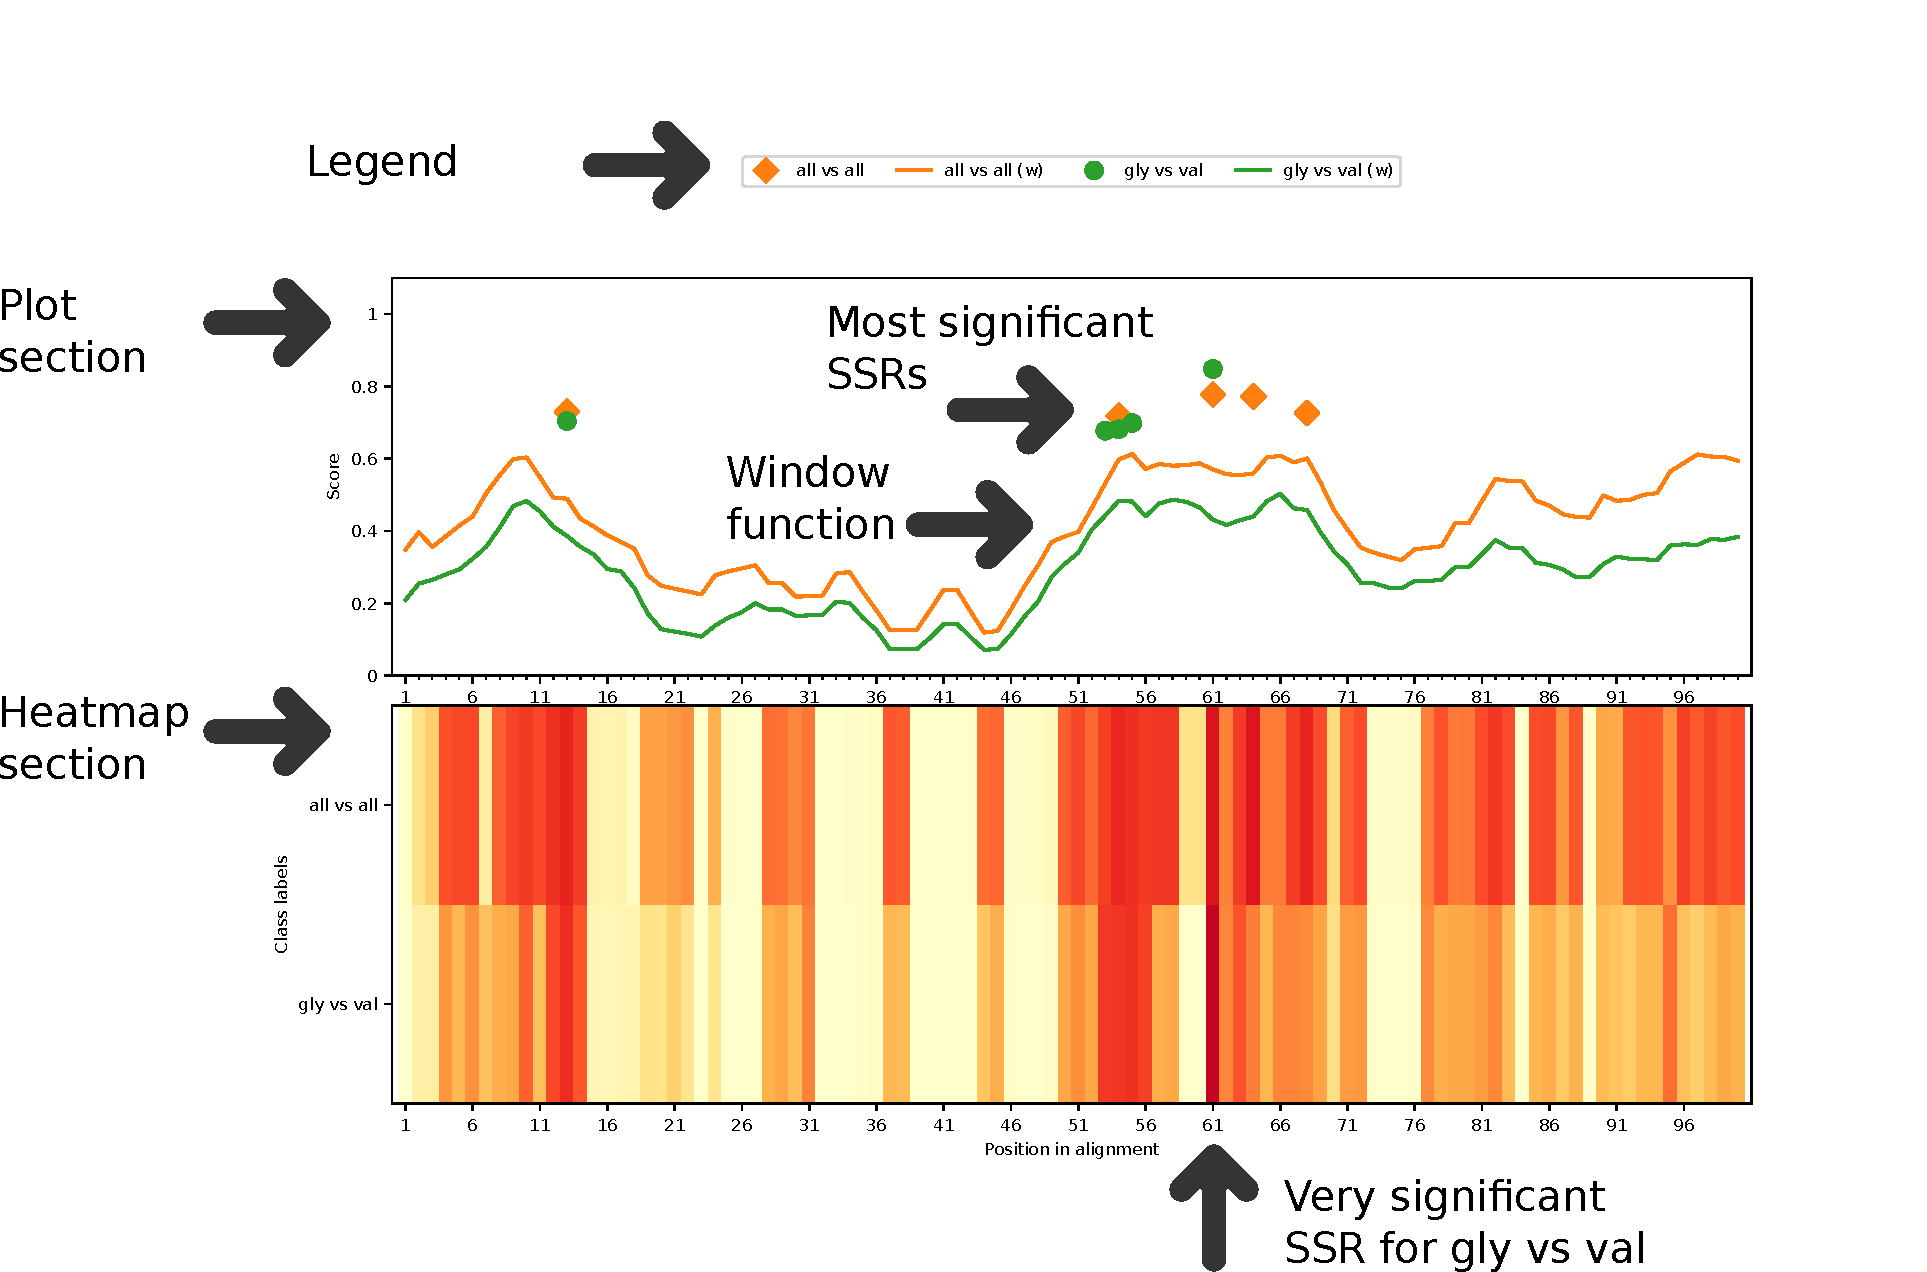
\includegraphics[width=\linewidth]{./figs/plot_example}
  \caption{Example SSR-viz output: The SSRs are computed for the adenylation domain of the NRPS system. 
  The subfamily classes are defined according to the substrate specificity of the domain: glycin (gly) and valine (val).
  See also the example in Section~\ref{example}.}
  \label{fig:plot_example}
\end{figure}

Keep in mind that for projects with multiple protein sub-families the plots can be 
easily overcrowded. A maximum of 10 panels for the heatmap and 5 panels for the plot are 
recommended.

\begin{description}

\item[\texttt{Remove label from top of plot}] \hfill \\

Usually a legend is plotted on top 
\todo{should be legend instead of label} of the plots, this looks only nice for about 5 or 6 labels.
It can be removed, but the recommended way is to plot the SSRs for less subfamilies. 

\item[\texttt{Figsize hight / Figsize width}] \hfill \\

The default figure size is Din A4 but any other size can be chosen.

\item[\texttt{Chunk size of the figure}] \hfill \\
 
How many residues should be plotted per page. 

\item[\texttt{Entire alignment in one plot}] \hfill \\

This argument would squeeze the entire alignment in one plot, 
which can be useful to get on overview of the alignment.

\item[\texttt{Tick positions}] \hfill \\

How often the positions should be shown in the bottom ticks.

\item[\texttt{Ratio plot / ratio heatmap}] \hfill \\

Sets the ration between plot and heatmap.

\end{description}

\subsubsection{Additional output}

Additionally to the created figure, two additional outputs can be created:

\begin{description}

\item[\texttt{Jalview annotation file}] \hfill \\

This file can be imported to Jalview, so that the SSR scores can 
be visualized together with the alignment. Just open the alignment with Jalview and 
click File, then Load Features/Annotations and then choose the created *.jv\_plot.txt 

\item[\texttt{Plot statistics}] \hfill \\

This creates a csv file, which shows tabular informations of the SSRs created. 
The file lists the significant positions for each scoring scheme, including the positions in the alignment,
the score, the conserved residue and the entire variety of residues for each subfamily. 

\end{description}

\subsubsection{Plot Options}

Here the plot output can be modified.

\begin{description}

\item[\texttt{Window size / Window type}] \hfill \\

Additionally to the most significant positions, the plot can also apply a window function to the SSRs.
This window function can be used to visualize general ares of interest in the alignment. 
Possible windows are: mean, max, min, std. 
If the window is set to 1 it shows you the exact SSRs for each residue.

\item[\texttt{No all vs all plot}] \hfill \\

Besides the chosen one-vs-one and one-vs-all schemes, the plot always shows the SSRs for the all-vs-all scheme, representing the residues
which are most important to distinguish all subfamilies from each other. This can be removed with this option.

\end{description}

\subsubsection{One-vs-One plot}

Here are all the subfamilies listed which were parsed from the subfamily class label CSV-file. 
Each subfamily can be chosen to compute the SSRs. Keep in mind, that an all-vs-all scheme can become very large, as each
subfamily will be compared to each other. Best practice would be to concentrate on a few (3-4) subfamilies and create multiple plots.

\subsubsection{One-vs-All plot}

The choice is identical to the One-vs-one plot, but shows most significant SSRs to distinguish each subfamily from all the other 
subfamilies.

\subsubsection{Heatmap Options}

\begin{description}

\item[\texttt{No all vs all row in the heatmap}] \hfill \\

Besides the chosen one-vs-one and one-vs-all schemes, the heatmap always shows the SSRs for the all-vs-all scheme, representing the residues
which are most important to distinguish all subfamilies from each other. This can be removed with this option.

\item[\texttt{Remove the labels from the heatmap}] \hfill \\

The labels can be removed from the heatmap. For example if very much one-vs-one schemes are shown, it looks better without labels.

\end{description}

\subsubsection{One-vs-One Heatmap}

Identical to One-vs-One plot, but for the heatmap.

\subsubsection{One-vs-all Heatmap}

Identical to One-vs-All plot, but for the heatmap.

\section{Add pdb} \label{add_p}

In order to simplify the observation of the detected SSRs in a structural context. This tool allows to assign
indices of a PDB file to the SSRs listed in the plot statistics CSV file ('stats.csv'). 
The offset (PDB structures are often shifted relative to
the original protein sequence) is adjusted (see Figure~\ref{fig:pdb_mapping}).  

Multiple PDB can be used, just change the \texttt{Input pdb file} and \texttt{Chain in the pdb file} argument as 
required and run the tool multiple times. If the input 'stats.csv' and the output 'stats.csv' are identical each run
will create a new row with PDB indices.

Note that if the mapping of the structure to the sequence leads to undesired results (for example
in case of a multi protein complex mafft does not know which part to align) it might be necessary to trim the 
PDB file to only contain the protein part that should be used. This can easily be done with pymol and is 
demonstrated in the use-case (see ~\ref{example})

\begin{figure}
  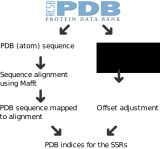
\includegraphics[width=\linewidth]{./figs/pdb_mapping}
  \caption{PDB mapping and offset adjustment scheme for the \textbf{Add\_pdb} tool.}
  \label{fig:pdb_mapping}
\end{figure}

\subsection{Arguments}

\begin{description}

\item[\texttt{Input sequence alignment}] \hfill \\

Input file must be a sequence alignment in FASTA format (the one used to create the plot statistics CSV file ('stats.csv')).

\item[\texttt{Input pdb file}] \hfill \\

Input file must be a PDB file which corresponds to the alignment (sequences should have a high similarity).
As long as the pdb and the original MSA can be aligned, the tool will do its job, but a reasonable output can
only be expected from a structure with reasonable sequence similarity.

\item[\texttt{Chain in the pdb file}] \hfill \\

Chain in the pdb file.

\item[\texttt{Temporary folder}] \hfill \\

Directory for the added alignment of the pdb and the mafft map file. This can also be the Folder where the other Outputs are stored.

\item[\texttt{Mafft executable}] \hfill \\

Mafft is used internally to add a sequence to an alignment.
In Linux if mafft is installed globally (it can be executed via the command line from anywhere), the default parameter
should be fine. In Windows one might have to search for the correct executable path (see~\ref{mafft}). 

\item[\texttt{Stats csv file}] \hfill \\

The indices of the PDB are added to the 'stats.csv' file created with SSR\_plot.

\item[\texttt{Output csv}] \hfill \\

Optional different output for the 'stats.csv' file, can be identical with the input file

\end{description}

\section{Use case} \label{example}

In the following example the adenylation domain of the nonribosomal peptide synthetases (NRPS) will be observed.
The substrate specificity of this domain is responsible for the high diversity of secondary metabolites of the 
type of nonribosomal peptides, a fast source for bioactive molecules such as antibiotics and cytostatics.
Further information can be found at: \url{https://en.wikipedia.org/wiki/Nonribosomal_peptide}.

All files needed to reproduce this example are provided in  \url{https://github.com/PhaBiFreiburg/SSR-viz/use_case}.

For this use case two subfamilies were
chosen, with respective specificities for valine and glycine. 
For both
subfamilies crystal structures are available (PDB: 3VNS, 4ZXI), so that
the detected SSRs can be interpreted in a structural context.

The sequences and subfamily labels were taken from Rausch \textit{et al.} \cite{rausch_specificity_2005}, one of the first comprehensive analyses of this domain.
The provided sequences were converted into a FASTA file using a simple Python Script. The original Data, the script and the FASTA
file can be found in \url{use_case/raw/a_doms/}.

\subsection{The clustering problem}

The provided example demonstrates why in many cases a clustering or phylogenetical analysis will not lead to
the desired subfamily grouping. The sequences are labeled according to their substrate specificity, which makes it 
easy to investigate the results of any clustering algorithm.

\begin{minted}{bash}
>Q9FDB3_m2_spec_pro # <- label
\end{minted}

The sequences were clustered using the default parameters of mafft.
If you want to reproduce the example, feel free to use the MSA tool of your choice.

\begin{minted}{bash}
mafft --auto NRPS_A_dom.fasta > NRPS_A_dom_ali.fasta
\end{minted}

For this alignment a phylogenetic tree was generated using the
web service of EMBL \url{https://www.ebi.ac.uk/Tools/phylogeny/simple_phylogeny/} with 
default parameters.

The resulting tree can be found in \url{use_case/raw/a_doms/phylo/A_dom_tree.txt.pdf}.
The carefully observation reveals, that even though some cases the sequences are clustered according to their specificity (see Figure~\ref{fig:cluster} (a)),
in most cases the clustering is rather based on evolutionary distance (see Figure~\ref{fig:cluster} (b)).

Therefore, 
if the desired subfamily class label definition is not 
directly associated with the evolutionary distance of the sequences,
an automated labeling approach will not lead to correct assignment.
Which means, that for best results in SSR detection the subfamily class label needs to be extracted from the literature
of experimentally derived labels.  

Nevertheless, SSR-viz can also be used for SSR detection of photogenically clustered sequences, if this 
is the desired clustering. 

\begin{figure}
  
\includegraphics[width=\linewidth]{./figs/cluster_good}
  \caption{Example of a phylogenetically clustering according to the substrate specificity.}
  \label{fig:cluster_good}
\end{figure}

\begin{figure}
  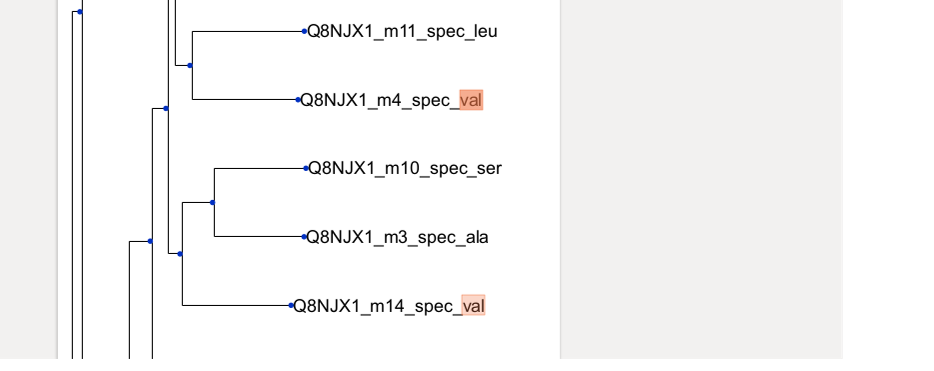
\includegraphics[width=\linewidth]{./figs/cluster_bad}
  \caption{Example of a phylogenetically clustering unrelated to the substrate specificity.}
  \label{fig:cluster_bad}
\end{figure}

\subsection{CSV builder}

Fortunately, for this example the subfamily class labels are already assigned and the sequences can be used to 
detect SSRs for the discrimination of sequences with specificity for for valine and glycine.

Therefore, additionally to the MSA a subfamily class label CSV needs to be created (see Figure~\ref{fig:csv_b_params}). 

\begin{figure}
  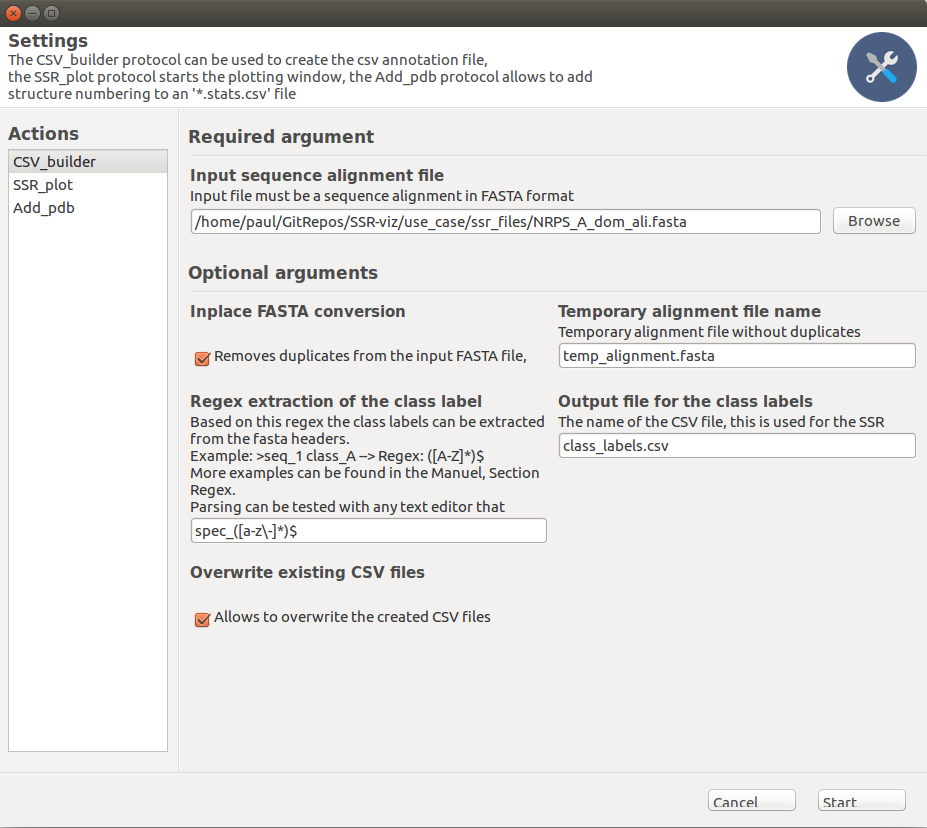
\includegraphics[width=\linewidth]{./figs/csv_b_params}
  \caption{Example of parameters used to create the subfamily class label CSV file.}
  \label{fig:csv_b_params}
\end{figure}

This could be a file with blank class labels, which need to be manually assigned. But as the class label can be found
in the FASTA sequence name tag, the Regex extraction routine can be used, which makes this task much easier.

\begin{minted}{bash}
>Q9FDB3_m2_spec_pro # <- label
\end{minted}

To design a working regex, the best option is to open the alignment in a text editor which supports Regex search and 
test if the class label can be found with the Regex string (see Figure~\ref{fig:subl_regex}). 

\begin{figure}
  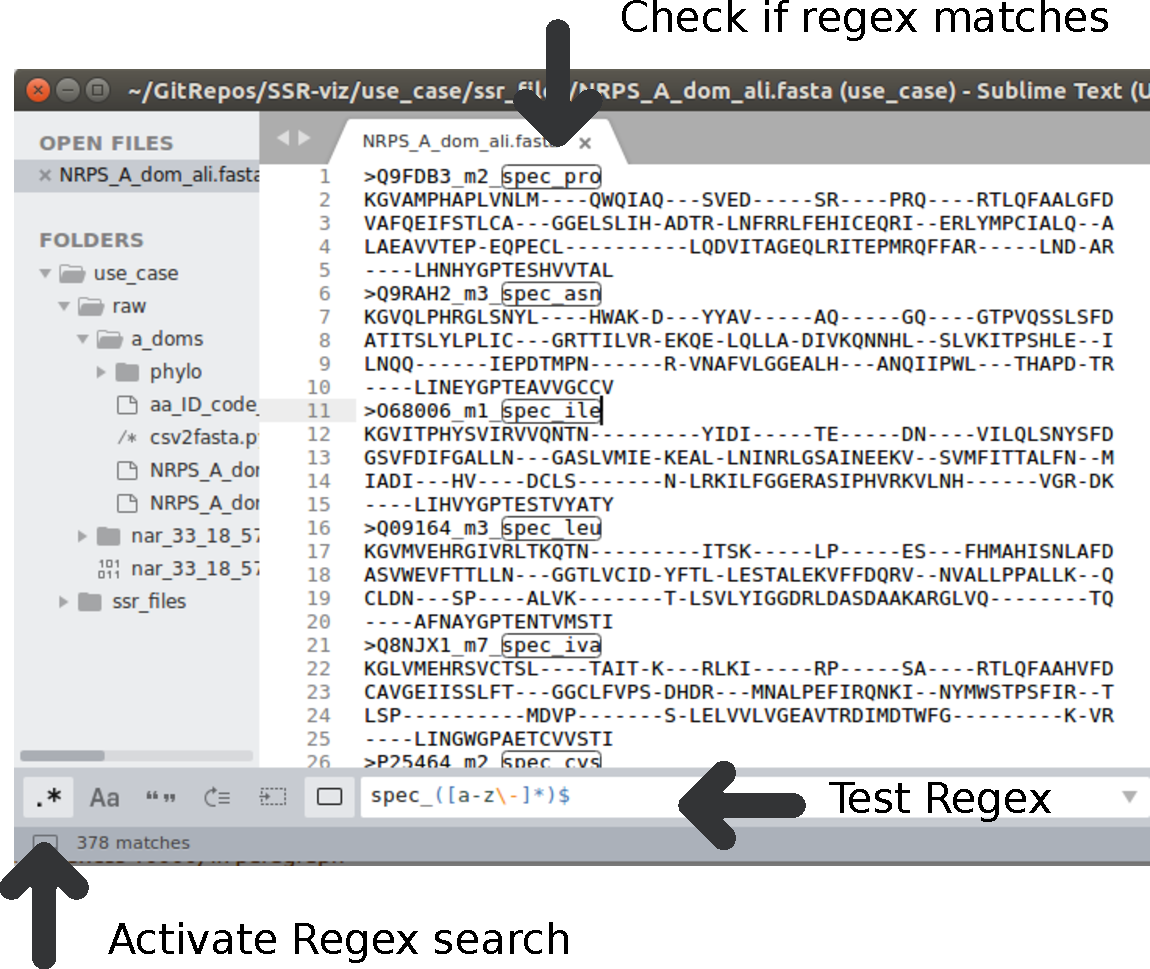
\includegraphics[width=\linewidth]{./figs/subl_regex}
  \caption{Usage of Sublime 3.0 to design the correct Regex for subfamily class label extraction.}
  \label{fig:subl_regex}
\end{figure}

It is important to create a Regex which can extract all possible labels. For example in this use case the
label might contain the sign '-', so this needs to be included into the Regex. 

\begin{minted}{bash}
>O33743_m1_spec_lys-b # <- label
\end{minted}

The \textbf{CSV\_Builder}
will in any case report, if the label for some domains could not be found (see Figure~\ref{fig:regex_fail}).
So in this example, a Regex which can also capture numbers would be better:

\begin{minted}{bash} 
spec_([0-9a-z\-]*)$
\end{minted}


\begin{figure}
  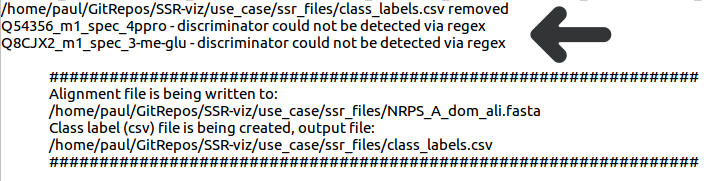
\includegraphics[width=\linewidth]{./figs/regex_fail}
  \caption{Example of labels, that could not be found with the regex, in this case, due to the missing number in the Regex.}
  \label{fig:regex_fail}
\end{figure}

If the label extraction was successfully, a file named class\_labels.csv should be created in the same folder as the MSA. 
This file should contain the corresponding subfamily class label for each sequence (see Figure~\ref{fig:class_labels}).
This file can be adjusted, for example if labels should be merged, changed or alternative labels should be used.
For alternative labels just add another column on the top row and add the desired labels (see Figure~\ref{fig:alter_label}).

\begin{figure}
  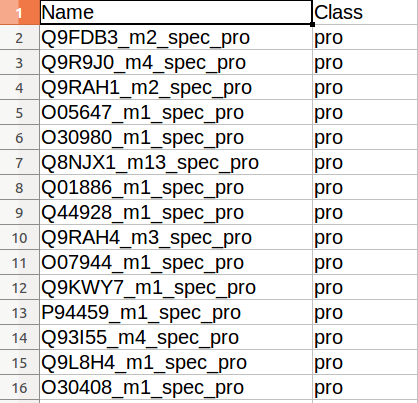
\includegraphics[width=\linewidth]{./figs/class_labels}
  \caption{Example of the subfamily class label CSV file.}
  \label{fig:class_labels}
\end{figure}

\begin{figure}
  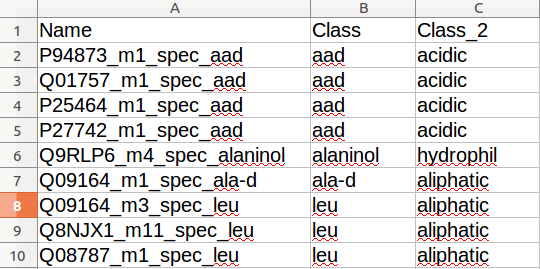
\includegraphics[width=\linewidth]{./figs/alter_label}
  \caption{In this example the alternative label assigns the amino acids to a higher hierarchical definition.
  This could be used to find SSRs responsible to discriminate proteins with specificity for aliphatic from proteins with specificity for 
  hydrophobic amino acids.}
  \label{fig:alter_label}
\end{figure}

\subsection{SSR plot}

The MSA and class label CSV file are now ready to be parsed by the \textbf{SSR\_plot} tool (see Figure~\ref{fig:ssr_plot}).

\begin{figure}
  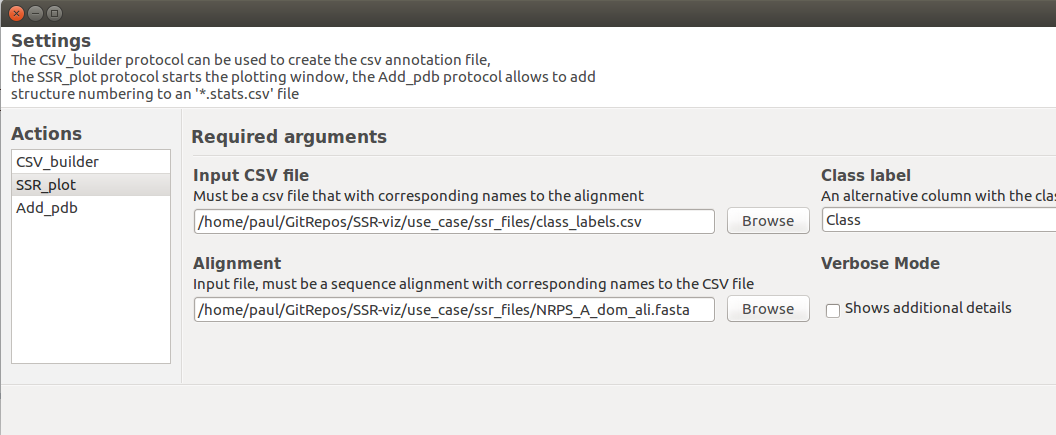
\includegraphics[width=\linewidth]{./figs/ssr_plot}
  \caption{Example of parameters used to parse the MSA and class label CSV file.}
  \label{fig:ssr_plot}
\end{figure}

If the files can be parsed a new window opens \textbf{SSR\_draw}.

\subsection{SSR draw}

In this window all parameters for the SSR detection and visualization can be adjusted (see Figure~\ref{fig:ssr_draw}). In this example the default parameters 
are chosen, which should be a good start for most analysis.

\begin{figure}
  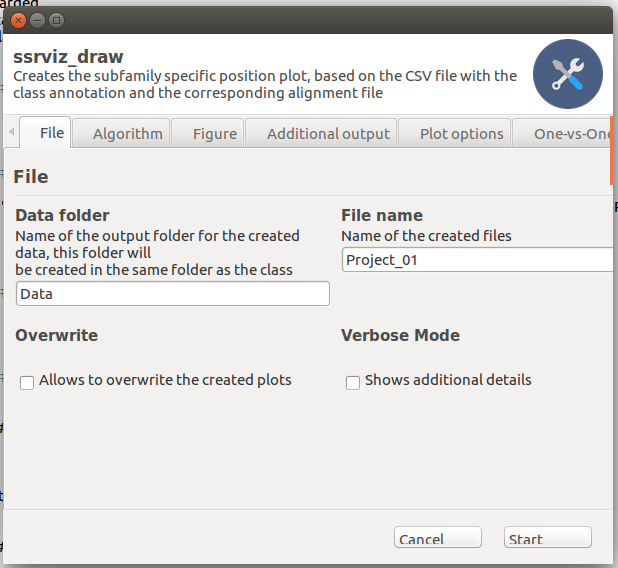
\includegraphics[width=\linewidth]{./figs/ssr_draw}
  \caption{Example of the \textbf{SSR\_draw} window.}
  \label{fig:ssr_draw}
\end{figure}

In order to demonstrate the full range of output options the Jalview Annotation File as well as the plot statistics file should be chosen as additional output 
(see Figure~\ref{fig:ssr_extra}).

\begin{figure}
  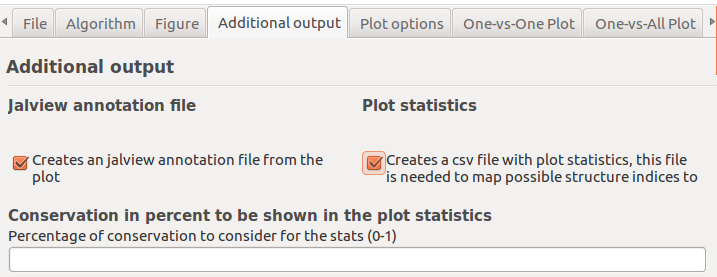
\includegraphics[width=\linewidth]{./figs/ssr_extra}
  \caption{Example of the additional output option.}
  \label{fig:ssr_extra}
\end{figure}

In order to visualize the differences for valine and glycine specificity those two subfamilies should be used as options for the
one-vs-one plot and heatmap options (see Figure~\ref{fig:label_choice}). Just scroll to the label and tick it.
Of course any other label could also be used.

\begin{figure}
  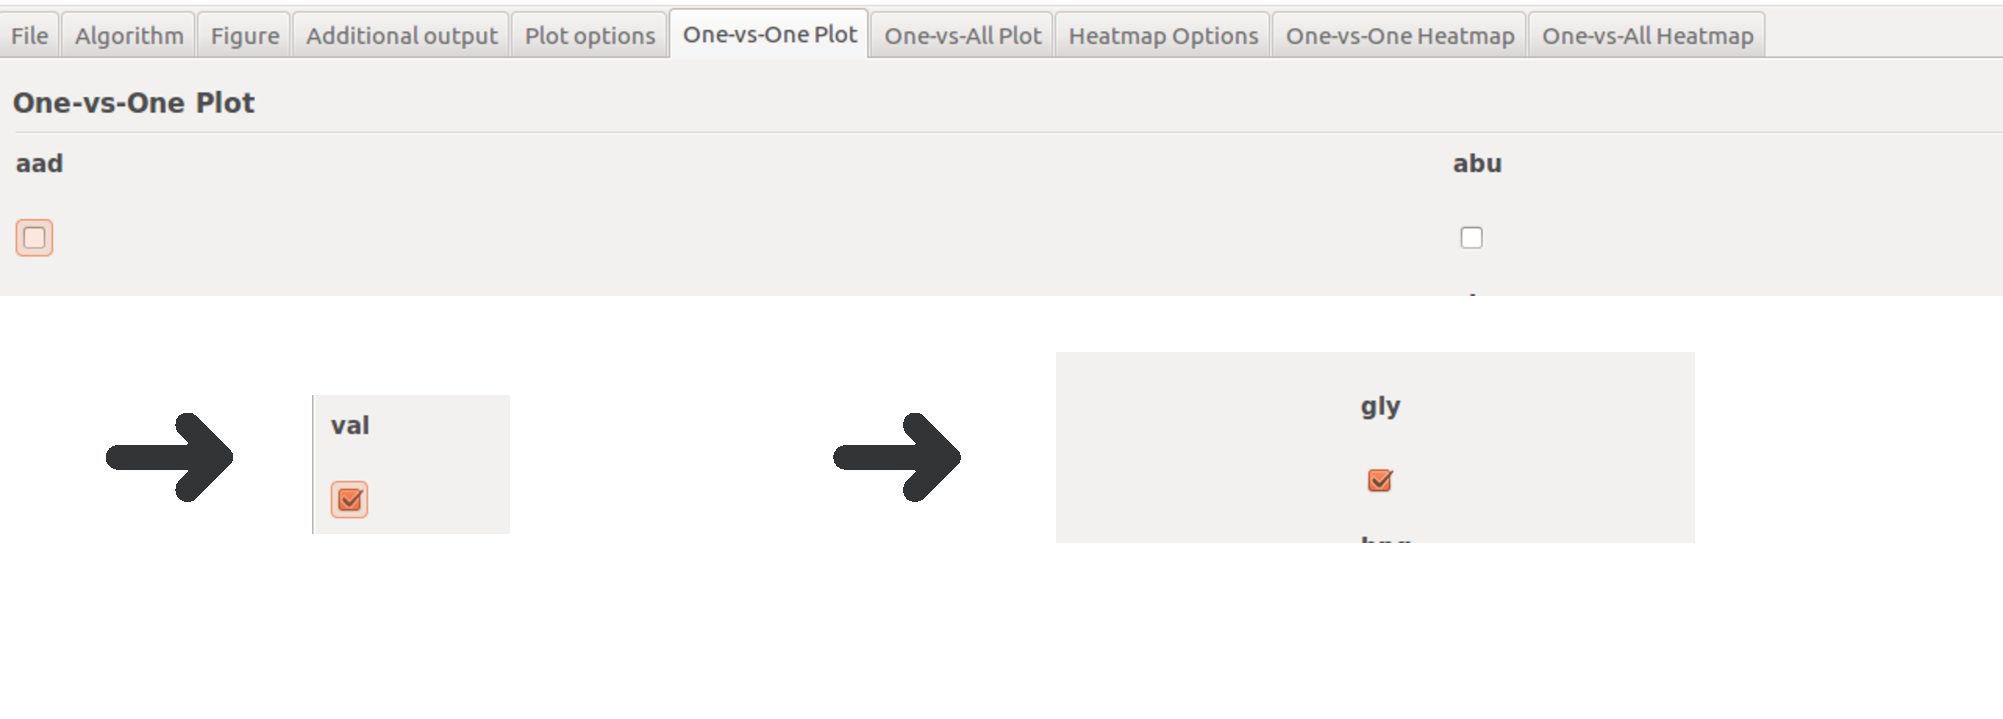
\includegraphics[width=\linewidth]{./figs/label_choice}
  \caption{Example of the label choice for valine and glycine specificity}
  \label{fig:label_choice}
\end{figure}

Start the program by clicking Start and if the program completes successfully, a new result folder named \textit{Data} should be created in the same folder as the MSA.

\subsection{Output}

In the results folder should be a plot called \textit{Project\_01.pdf}, which shows the results of the SSR detection in form of a plot and a heatmap as 
described in Figure~\ref{fig:plot_example}. This plot can be used to gain an overall impression of the SSRs for the chosen subfamilies. 

In this example,
the SSRs for two subfamilies are shown alongside the SSRs for all the subfamilies. Some positions overlap, for example position 61 is 
very important to distinguish all the subfamilies from each other as well as the two subfamilies (this position is probably in the center of the active cite !).
Other positions are only important for the two subfamilies. And again some positions are generally important for the substrate choice, but are of low significance for these
two families.
Additionally, the plot of the window function highlights general areas of interest. 
The first page of the plot is always a summary of the used parameters as shown in Figure~\ref{fig:plot_page1}.

\begin{figure}
  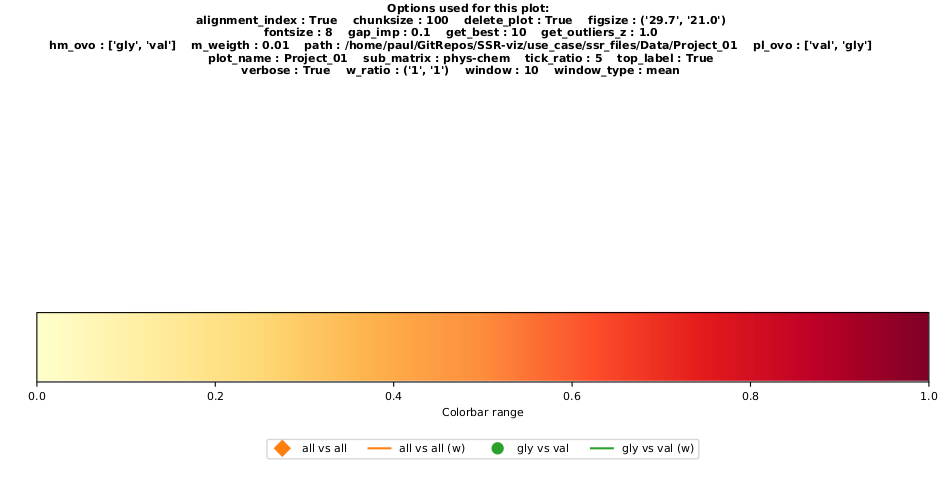
\includegraphics[width=\linewidth]{./figs/plot_page1}
  \caption{Example of the parameters page for the use case.}
  \label{fig:plot_page1}
\end{figure}

In many cases it is useful to observe the detected SSRs in the context of the alignment, therefore the file 'Project\_01\_jv\_plot.txt' is created,
which can be loaded into the Jalview alignment editor (see Figure~\ref{fig:JV_ali}). This allows to investigate the 
SSRs together with the vast toolbox of the Jalview editor.

\begin{figure}
  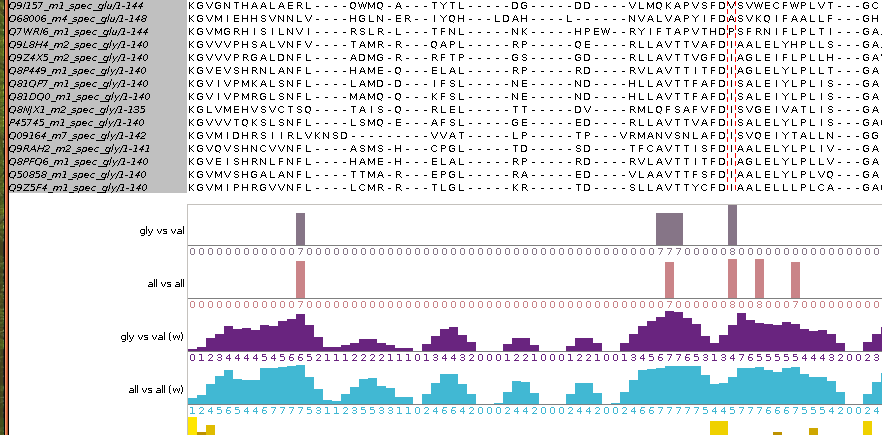
\includegraphics[width=\linewidth]{./figs/JV_ali}
  \caption{Example of the Jalview annotation file loaded into Jalview, together with the original alignment. Position 61 is marked. The proteins
  with specificity for glycine, show a conserved isoleucine at this position.}
  \label{fig:JV_ali}
\end{figure}

A summary of the mot significant SSRs can be found in the plot statistics CSV file 'Project\_01\_stats.csv'. This file shows the most significant 
SSRs for all the schemes chosen in the plot options (see Figure~\ref{fig:plot_stats}). Additionally the conserved residue (Cons) of each subfamily
for the SSRs are shown, as well as the full choice of residues (All res.).

\begin{figure}
  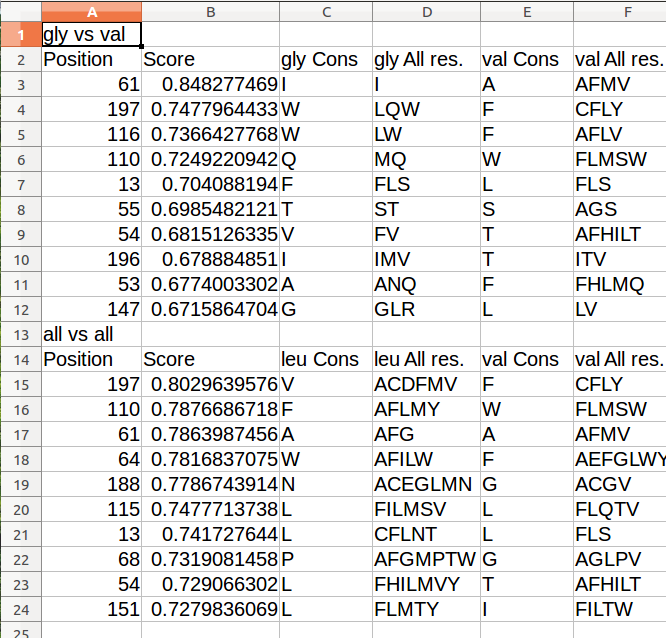
\includegraphics[width=\linewidth]{./figs/plot_stats}
  \caption{Example of the plot statistics CSV file. The top 10 SSRs are shown for subfamilies with specificities for glycine and valine, 
  as well as all the subfamilies. Whereas many positions overlap, position 116 is only of high relevance for the two subfamilies.}
  \label{fig:plot_stats}
\end{figure}

\subsection{Add pdb}

If structures of the observed proteins are available, it is often desired to investigate the detected SSRs in a structural context.
Theoretically, this could be achieved by using Jalview, as it supports the inclusion of structures to the MSA, but many users 
prefer a sophisticated protein viewer like pymol, which requires the mapping of any structure to the MSA.
Therefore, a simple routine was implemented which allows to map the indices of a PDB file to the SSRs in the plot statistics CSV file.

For this example the PDBs of a member of the subfamily with glycine specificity (PDB: 4zxi) as well as valine specificity (PDB: 3vns) were used.
Additionally, the structure (PDB: 1amu) was added, as this is the structure where Stachelhause \textit{et al.} \cite{stachelhaus_specificity-conferring_1999} based their investigation upon, which  
allows an easy comparison of the detected SSRs with the proposed specificity-conferring code. 
An example of the parameters used to map the indices are shown in Figure~\ref{fig:Add_pdb}.

\begin{figure}
  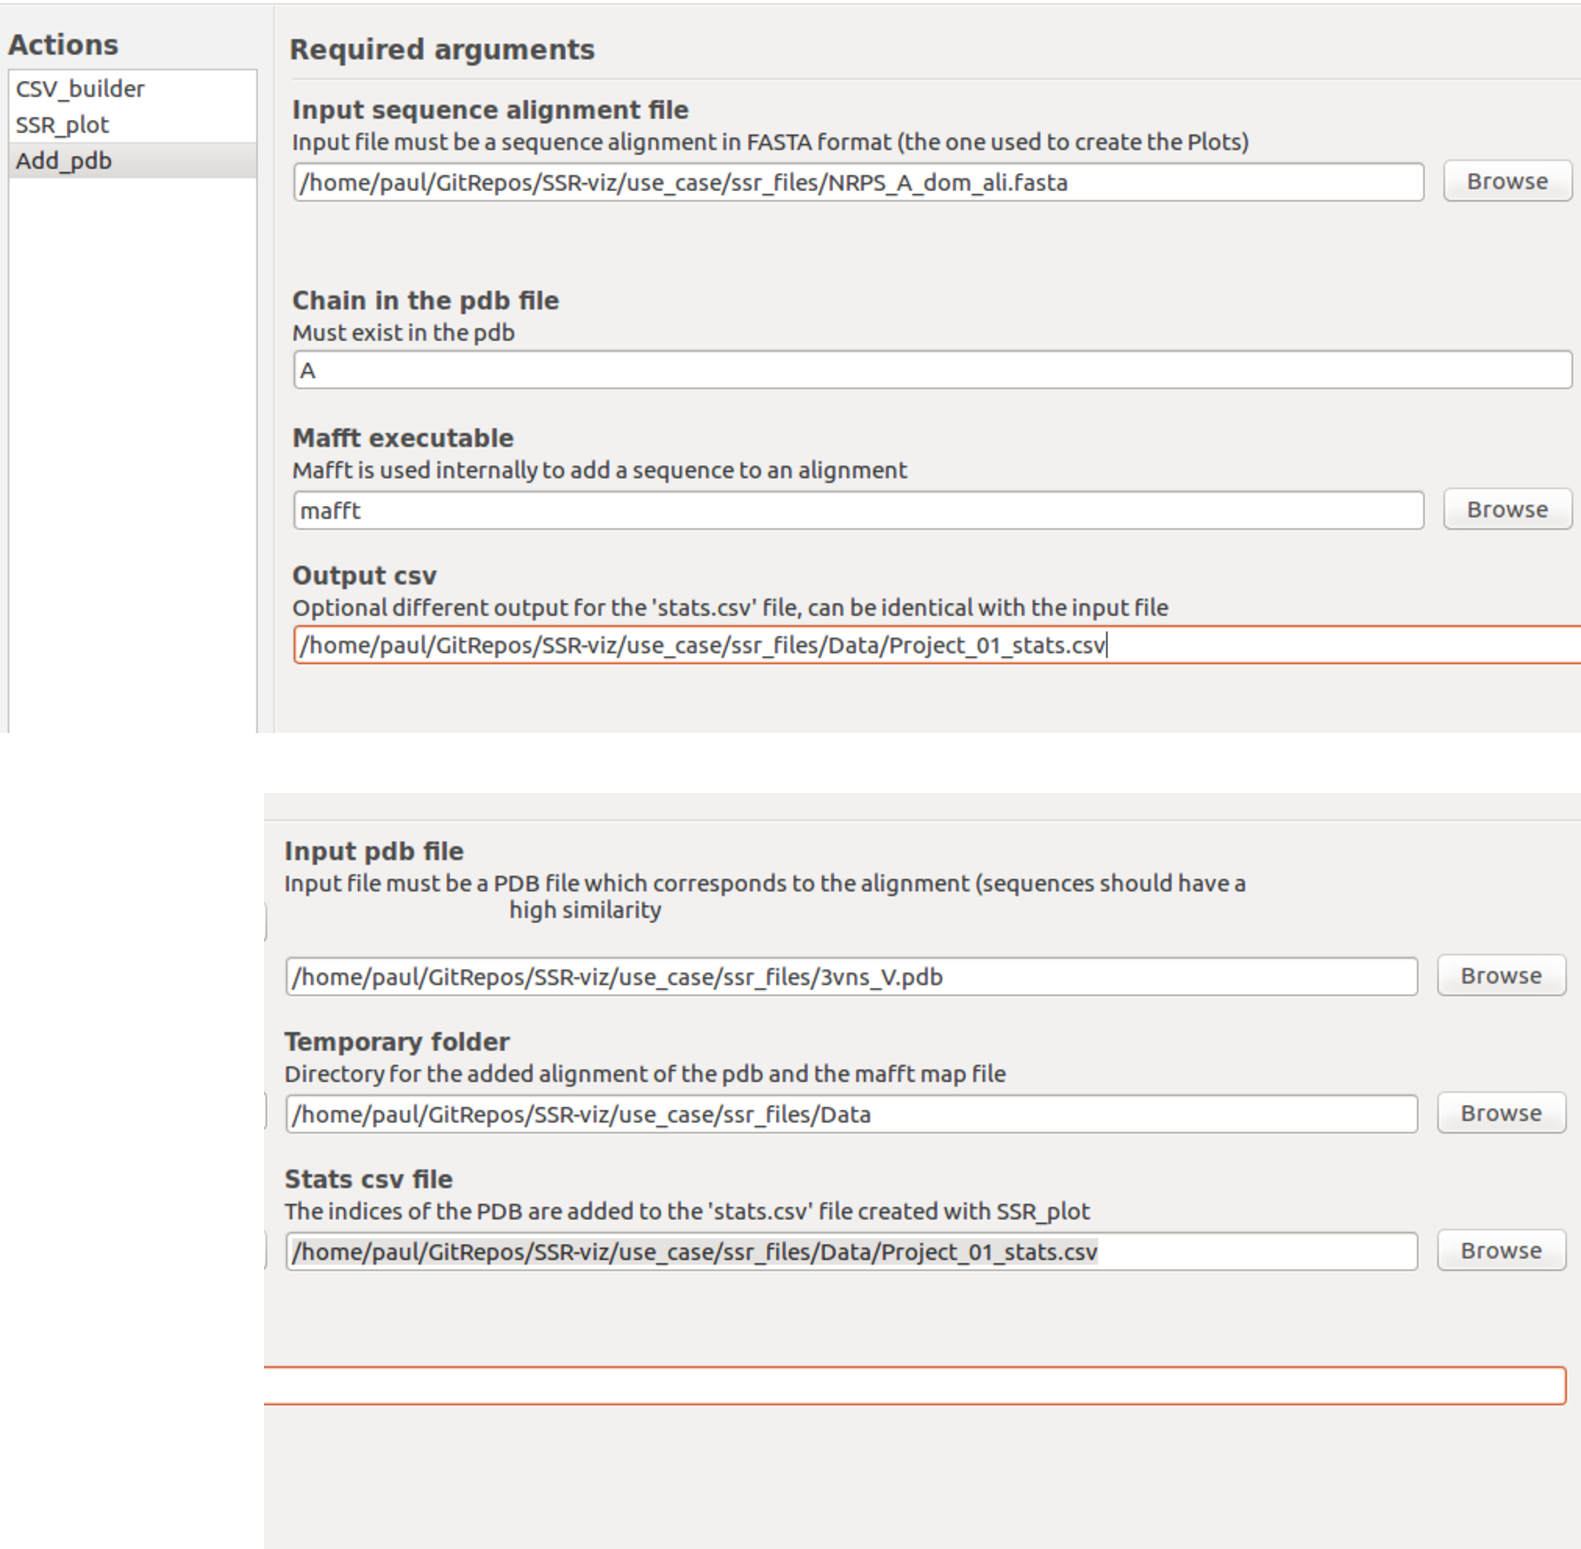
\includegraphics[width=\linewidth]{./figs/Add_pdb}
  \caption{Parameters used to map the indices of 3vns to the MSA.}
  \label{fig:Add_pdb}
\end{figure}

If the tools finishes successfully the indices of the structure are added to the plot statistics CSV file (see Figure~\ref{fig:added_pdb}).

\begin{figure}
  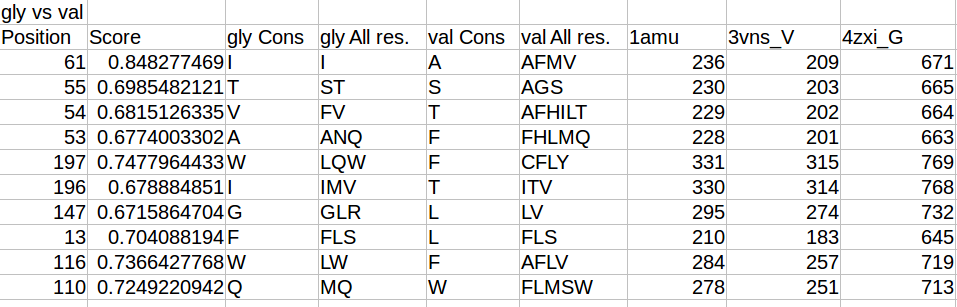
\includegraphics[width=\linewidth]{./figs/added_pdb}
  \caption{PDB indices added to the plot statistics CSV file}
  \label{fig:added_pdb}
\end{figure}

\subsection{Results}

Now that all the outputs are created and structure indices are added the detected SSRs can be investigated.
Lets have a look at the SSRs detected for the two subfamilies. This can for example be achieved by 
loading the PDB into pymol and selecting the SSRs with a command such as:

\begin{minted}{bash} 
select 3vns and resi 209+203+202+201+315+314+274+183+257+251
\end{minted}

The SSRs detected for each subfamily are shown in the respectively structure in Figure~\ref{fig:G_res} and Figure~\ref{fig:V_res}.
All SSRs are in close proximity to the substrate as expected for the specificity defining residues. Interestingly, only 4 residues 
directly interact with the substrate. The overlap of the SSRs for both subfamilies are shown in Figure~\ref{fig:positions}.
Position 331 and 236 (based on 1amu numbering) are the most significant SSRs for those two subfamilies, 
which can be explained trough steric interaction with the substrate.

\begin{figure}
  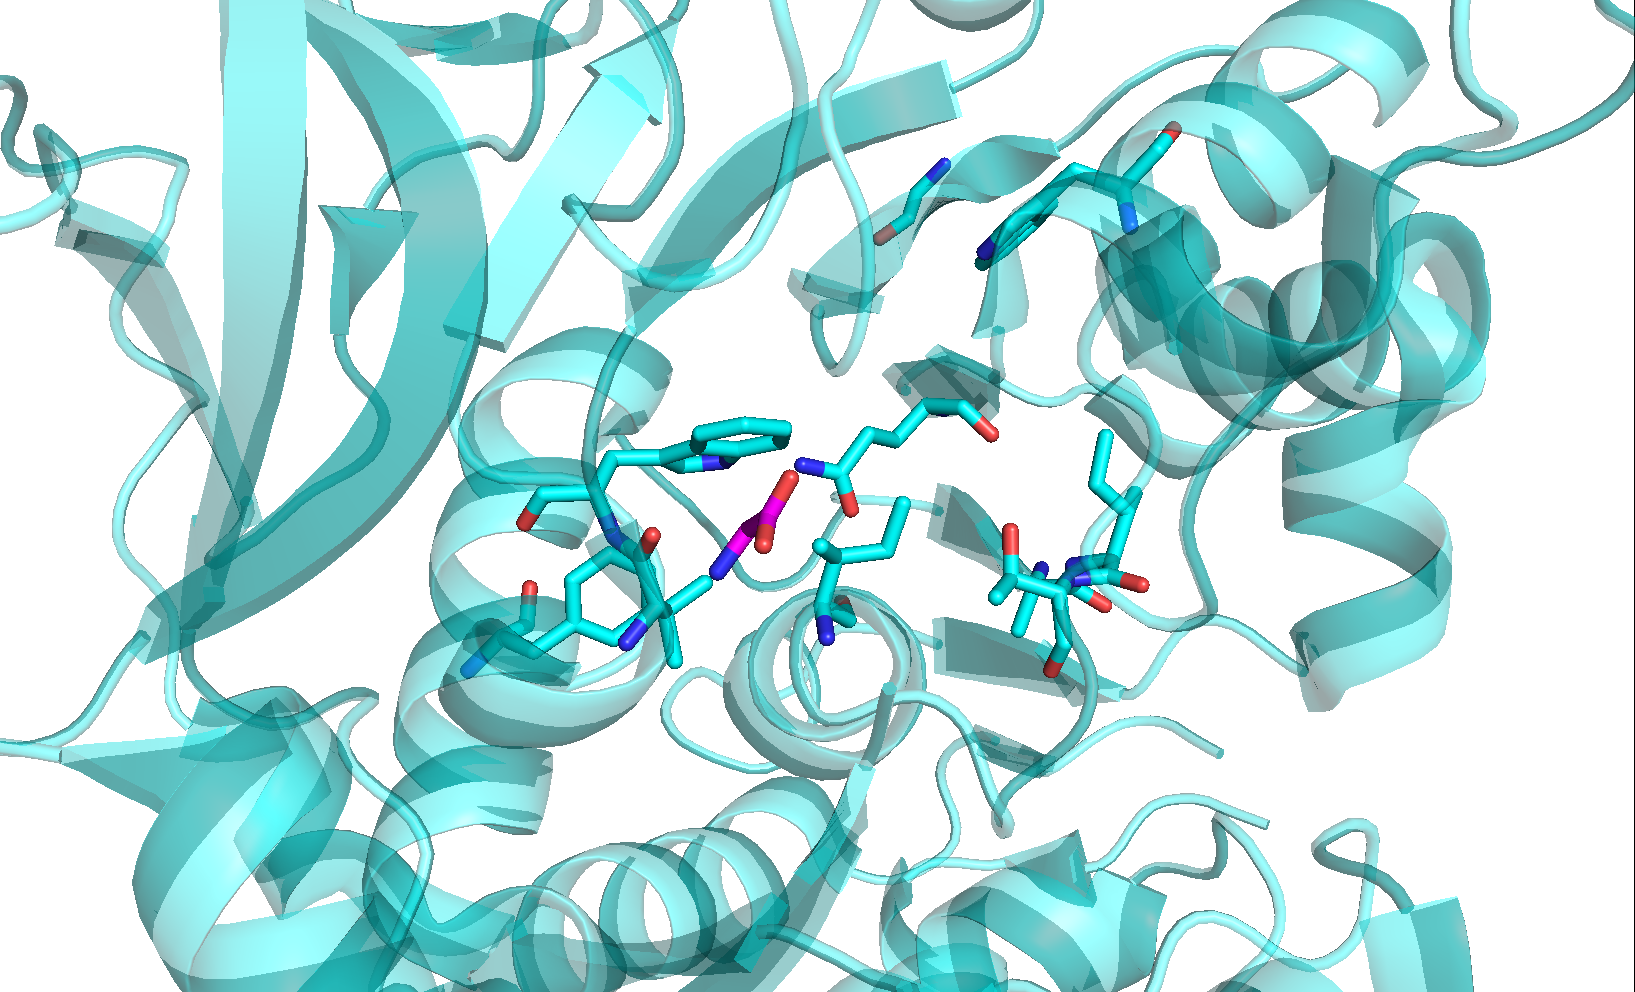
\includegraphics[width=\linewidth]{./figs/G_res}
  \caption{SSRs for 4zxi with specificity for glycine}
  \label{fig:G_res}
\end{figure}

\begin{figure}
  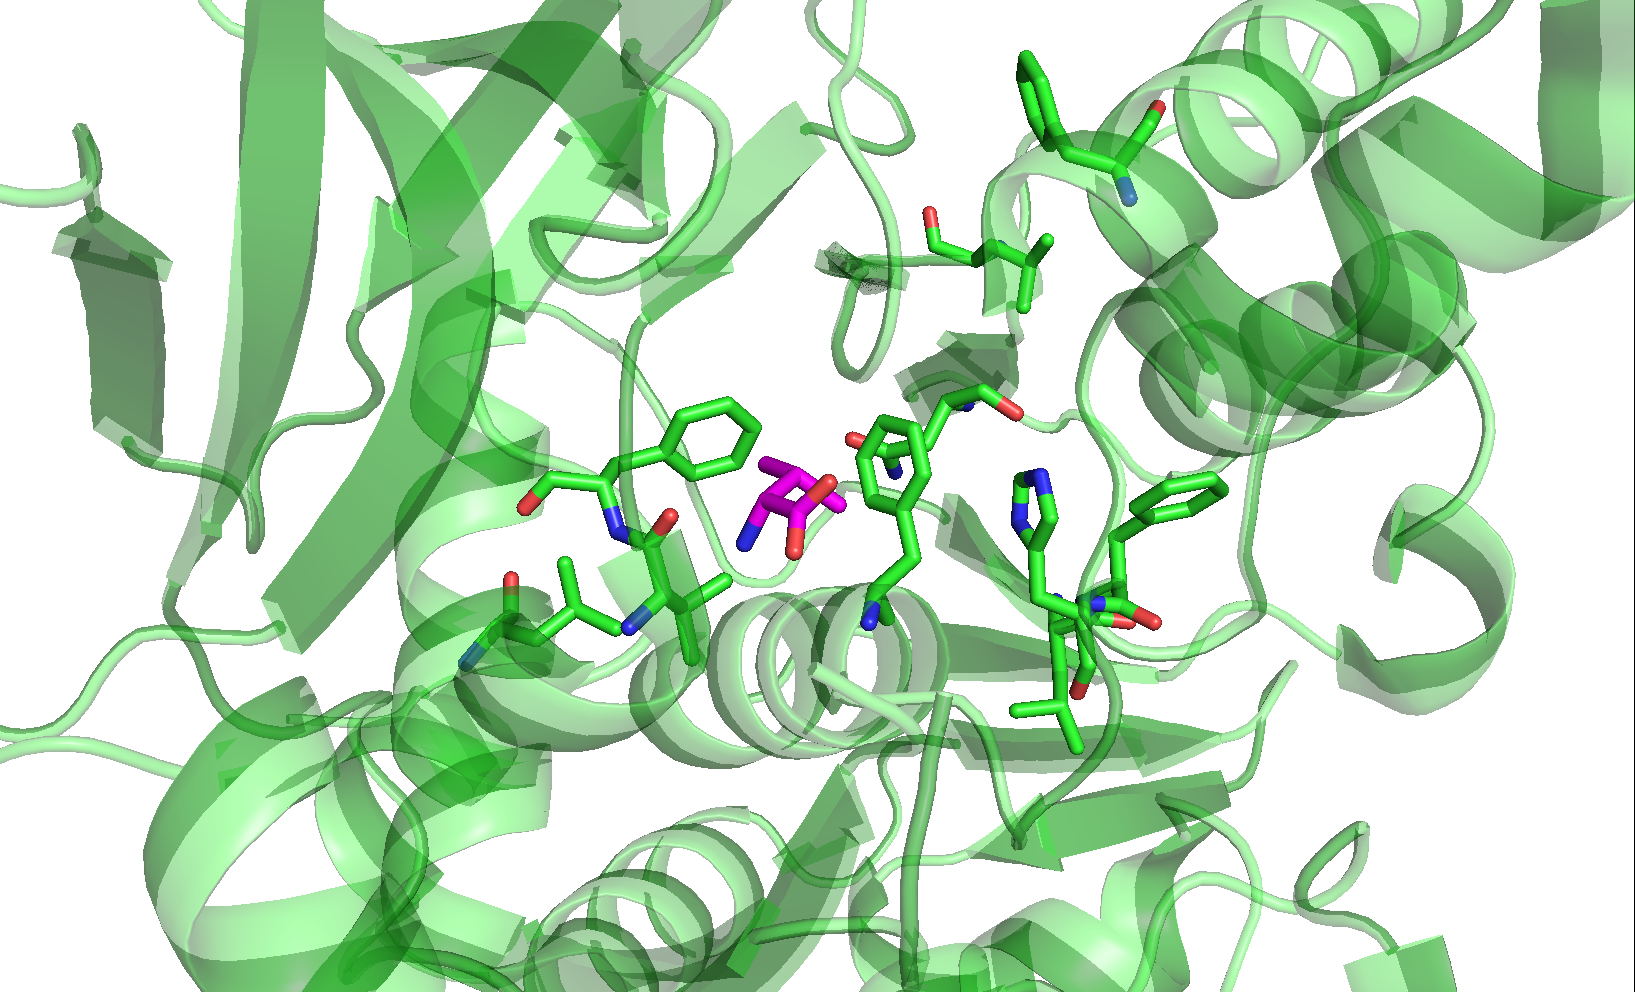
\includegraphics[width=\linewidth]{./figs/V_res}
  \caption{SSRs for 4zxi with specificity for valine}
  \label{fig:V_res}
\end{figure}

\begin{figure}
  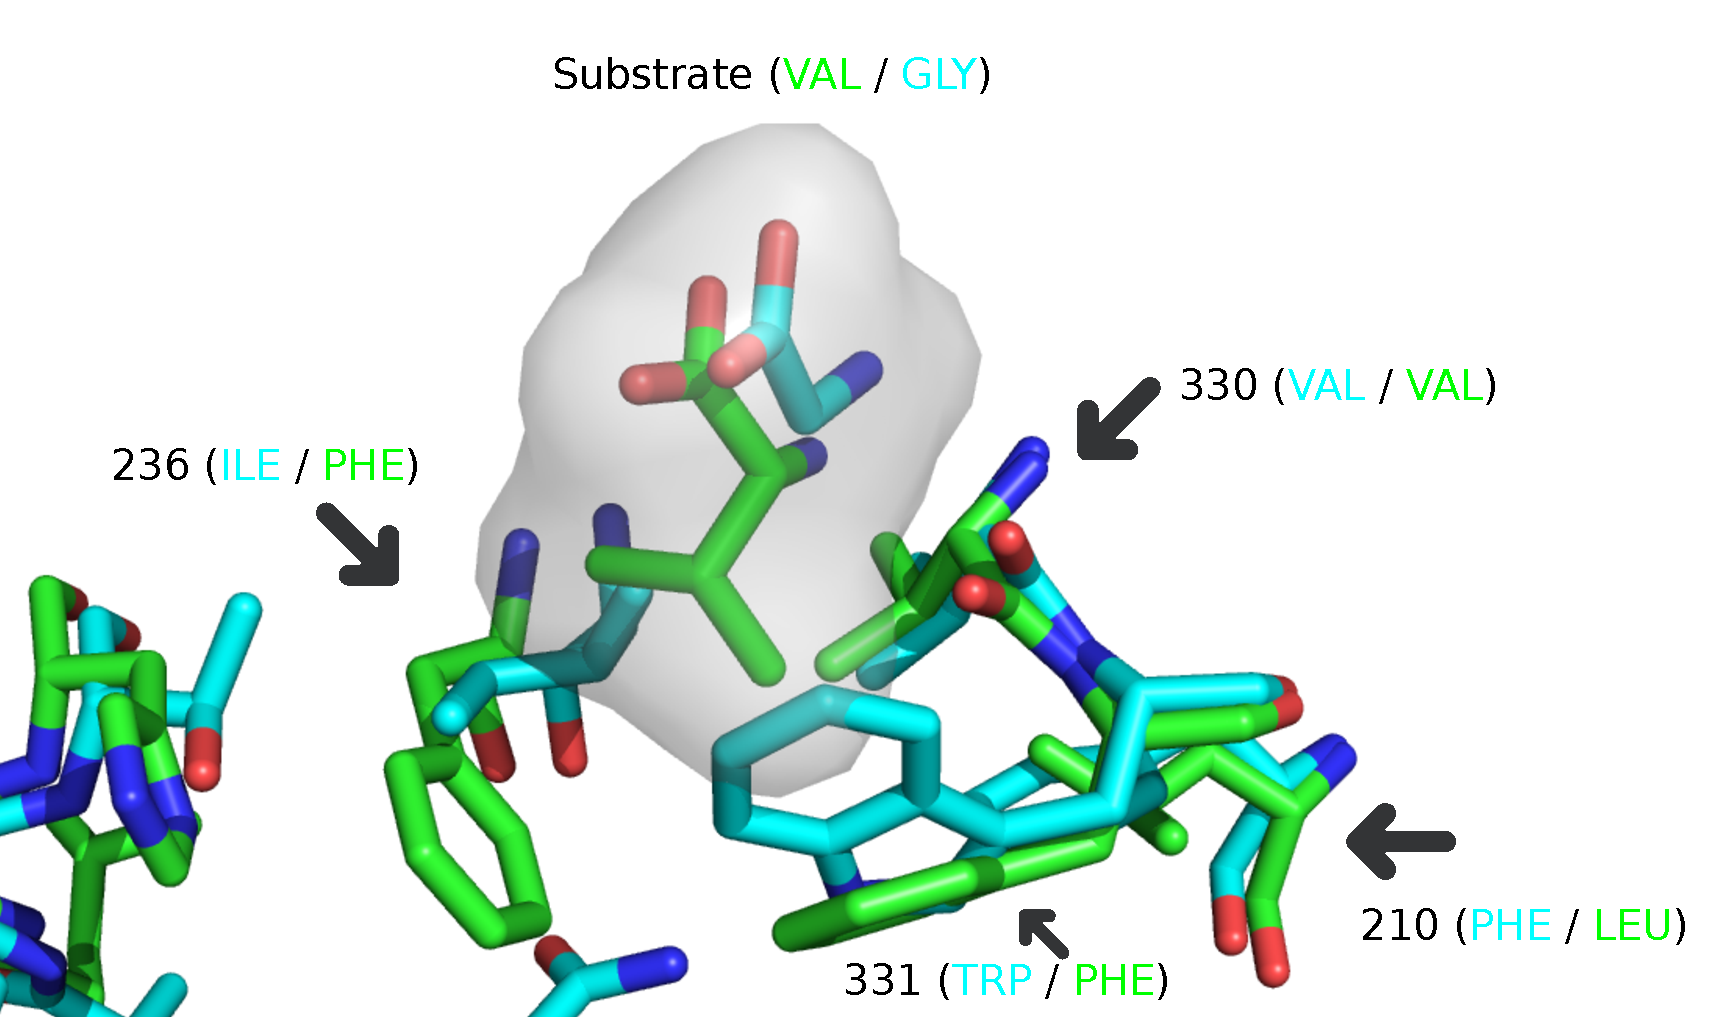
\includegraphics[width=\linewidth]{./figs/positions}
  \caption{Overlap of the SSRs in close proximity to the substrate.}
  \label{fig:positions}
\end{figure}

The SSRs for the all-vs-all scoring scheme can be compared with the observations of Stachelhause \textit{et al.} \cite{stachelhaus_specificity-conferring_1999}
as the most significant SSRs for all the subfamilies should correlate with the proposed specificity-conferring code.

In the proposed specificity-conferring code the residues are divided into highly variant and moderately variant residues.
Of the detected SSRs all the highly variant residues are included in the top 10 SSRs (239, 278, 299, 322, 331 
(based on 1amu numbering)). 

\subsection{Conclusion}

The detected SSRs can explain the substrate choice of the investigated protein subfamilies. Also, the SSR analysis 
of the entire family is in good accordance with proposed position of the literature, demonstrating the general applicability of SSR-viz. 

Feel free to further investigate the provided adenylation domain example. For example, it can be experimented how the subfamilies with specificity for aliphatic
amino acids are distinguished from each other. Or the One-vs-All scheme can be explored by investigating how any subfamily is distinguished from all the others.

If you have your own project feel free to explore the SSRs of a given problem using the entire range of SSR-viz.

\section{Appendix} \label{appendix}

\subsection{How to install and set up Mafft} \label{mafft}

Mafft is needed as the alignment tool used to map the PDB indices to the MSA. Therefore, SSR-viz can in 
general work fine without mafft, but if the \textbf{Add\_PDB} tool is needed mafft needs to be installed.

\subsubsection{Linux}

For Linux mafft can be installed very easy, just type 

\begin{minted}{bash} 
sudo apt install mafft
\end{minted}

Or check on their homepage 
\url{https://mafft.cbrc.jp/alignment/software/}
for other installation options.

If the installation is done, one should be able to call mafft with:

\begin{minted}{bash} 
mafft input > output
\end{minted}

In this case the default mafft executable path should be fine.
If for some reason mafft is stored in another place, the path needs to be adjusted.

\subsubsection{Windows}

In windows the tested way to get mafft working is to 
install mafft as described in \url{https://mafft.cbrc.jp/alignment/software/windows_without_cygwin.html}.
As this is an all-in-one package, one basically only needs to download the .zip file and unpack it and 
mafft is up and running.

To use mafft in SSR-viz, the 'mafft.bat' file needs to be selected as mafft executable path (see Figure~\ref{fig:mafft_windows}).
To simplify things it makes sense to unpack the mafft .zip file inside the SSR-viz folder. 

\begin{figure}
  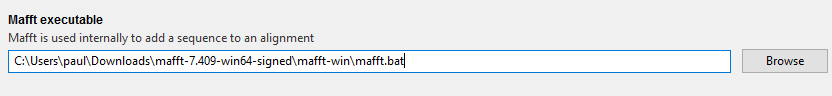
\includegraphics[width=\linewidth]{./figs/mafft_windows}
  \caption{Example of the mafft executable path.}
  \label{fig:mafft_windows}
\end{figure}

\subsection{Regex examples}

If sequences are download from the literature or created from other sources using a script, 
they probably contain the subfamily class label information somewhere in their FASTA name tag.
Here are some examples of possible names and how to extract the subfamily class label using regex.
Keep in mind that brackets () are used to define the part which should be extracted. \\

\begin{tabular}{|p{4.5cm}|p{4cm}|p{2cm}|}
\hline
Seq. name & Regex & Label \\
\hline
>sequence1\_spec\_ADP \newline >sequence2\_spec\_ATP & \verb|_spec_([A-Z]*)$| & ATP \newline ADP \\
\hline
>sequence1\_1 \newline >sequence2\_2 & \verb|_([0-9]*)$| & 1 \newline 2 \\
\hline
>ASH1L-1\_Class:0 \newline >ATAD2-1\_Class:1 & \verb|Class:([0-9]*)$| & 0 \newline 1 \\
\hline
>Q9FDB3\_m2\_spec\_pro \newline >Q00869\_m1\_spec\_hyv-d & \verb|_spec_([A-Z\-]*)$| & pro \newline hyv-d \\
\hline
>AT\#Alpha\#0030\#m \newline >AT\#Alpha\#0020\#mm & \verb|\#[a-z]*)$| & m \newline mm \\
\hline
>AB-sequence1 \newline >AK-sequence1 & \verb|^[A-Z]*\-| & AB \newline AK \\
\hline
\end{tabular}


\printbibliography 

\end{document}
